\documentclass[letterpaper,12pt]{article}
\usepackage{tabularx} % extra features for tabular environment
\usepackage{amsmath}  % improve math presentation
\usepackage{float}
\usepackage{pdfpages}

\usepackage{graphicx} % takes care of graphic including machinery
\graphicspath{ {./figures/} }
\usepackage[margin=1in,letterpaper]{geometry} % decreases margins
\usepackage{cite} % takes care of citations
\usepackage[final]{hyperref} % adds hyper links inside the generated pdf file
\hypersetup{
	colorlinks=true,       % false: boxed links; true: colored links
	linkcolor=blue,        % color of internal links
	citecolor=blue,        % color of links to bibliography
	filecolor=magenta,     % color of file links
	urlcolor =blue         
}

%



\begin{document}

\title{Experiment 5 Preliminary Work \protect\\ Operational Amplifiers}
\author{Ahmet Akman 2442366 \protect\\}
\date{\today}
\maketitle

%\begin{abstract}
%abstract
%\end{abstract}

\section{Introduction} 
In preliminary work of the Experiment 5 , the steps for the pre-experiment are conducted and presented.
\section{Step 1}
Videos in  ODTUCLASS related to this experiment is watched and observations are noted.
\section{Step 2}
"Notes on Op-Amps" documents is studied.
\section{Step 3}
In this step following 4 op-amp circuits are constructed in the LTSpice environment and simulated. \(V_{in (t)}\) is taken as \(3sin(1000\pi)\) Volts. Then data are fetched from LTSpice and plotted in MATLAB.
\subsection{a)}
Basic comparator circuit is constructed in LTSpice environment. The schematic is given in the Figure 1.
\begin{figure}[H]
	\centering
   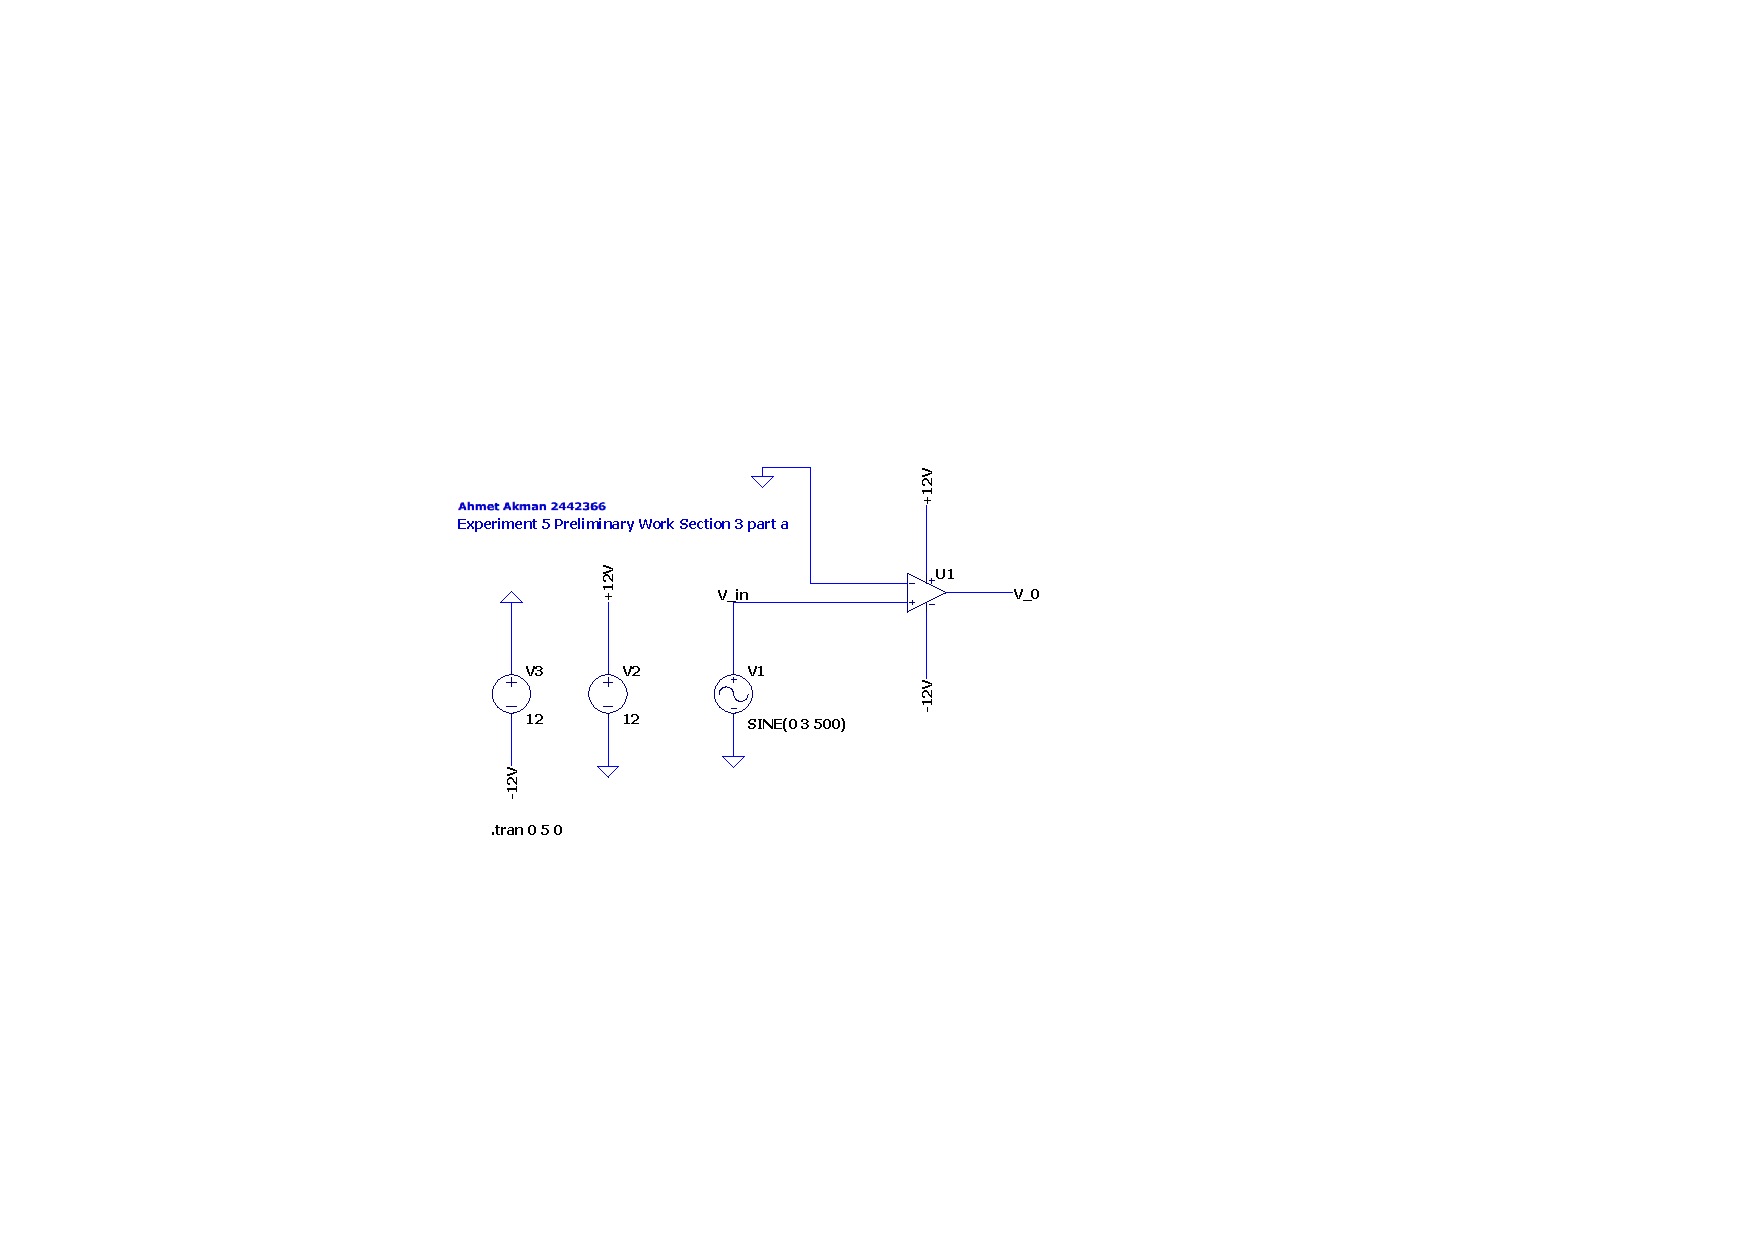
\includegraphics[width=0.8\textwidth]{BasicComparator_SCH.pdf}
   \caption{Circuit schematic for the basic comparator.}
\end{figure} 
Then plots given in Figures 5,6 and 7 are obtained.
\begin{figure}[H]
	\centering
   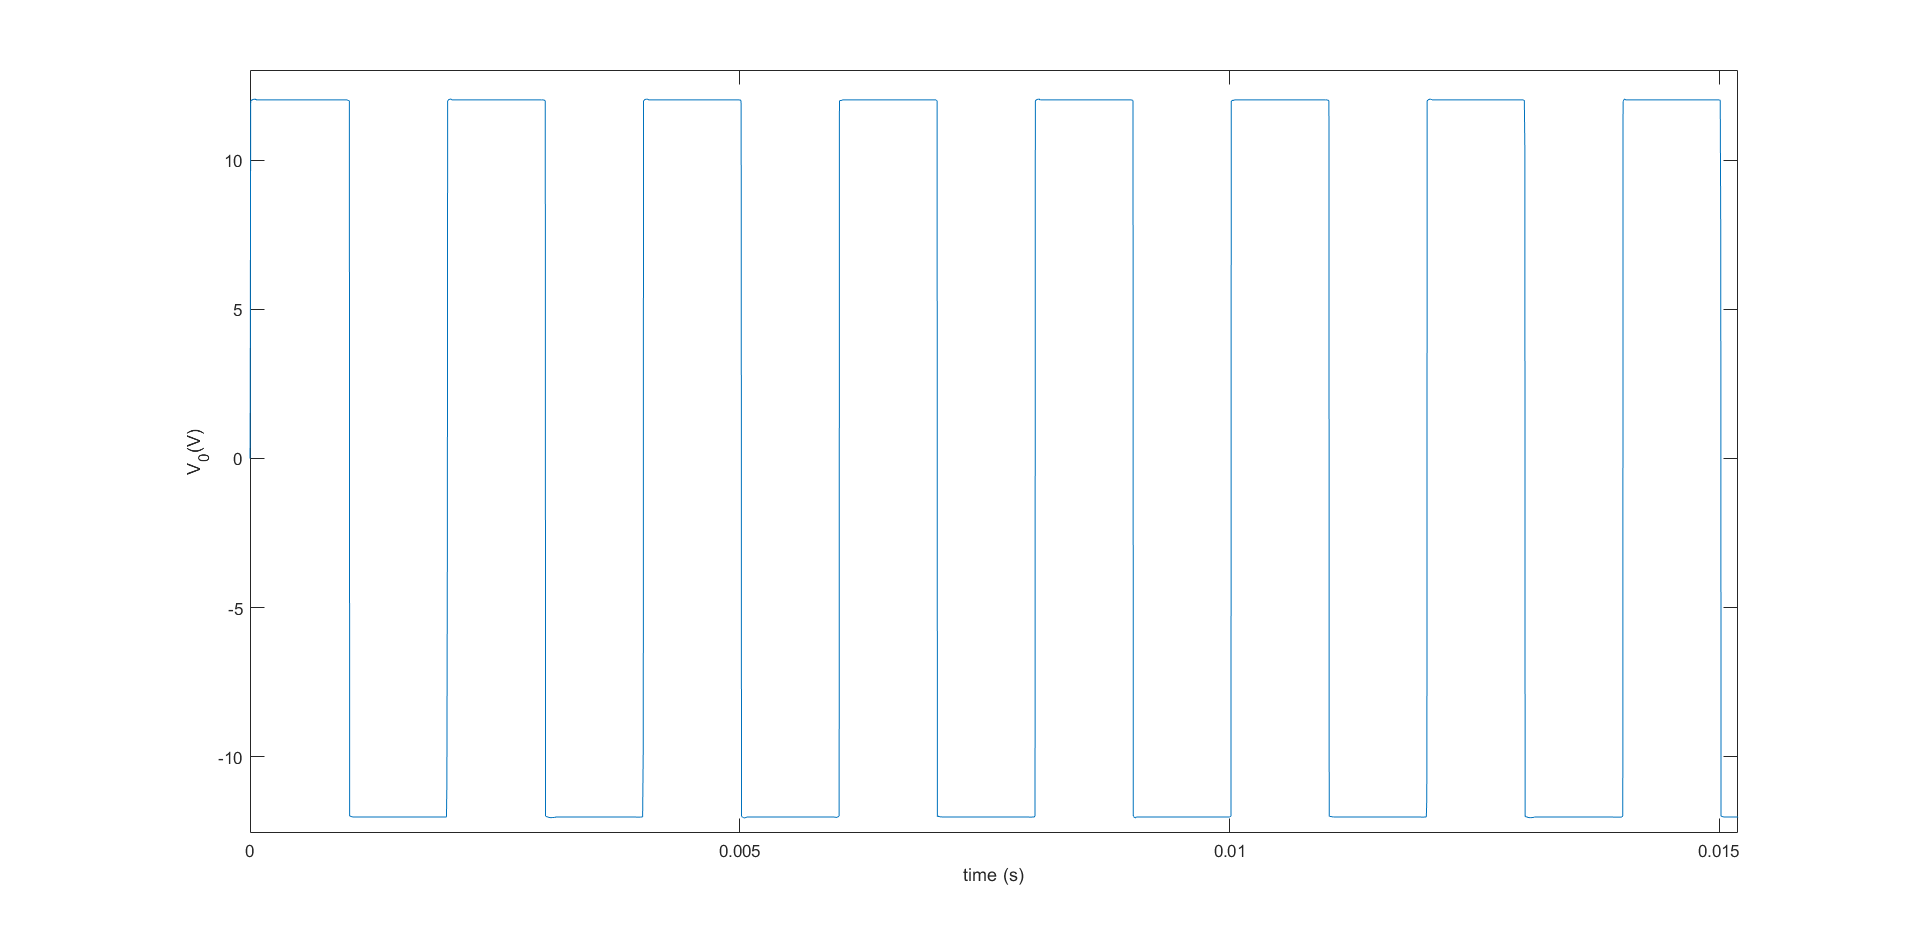
\includegraphics[width=1\textwidth]{3a_vs_t.png}
   \caption{\(V_0\) vs t}
\end{figure}

\begin{figure}[H]
	\centering
   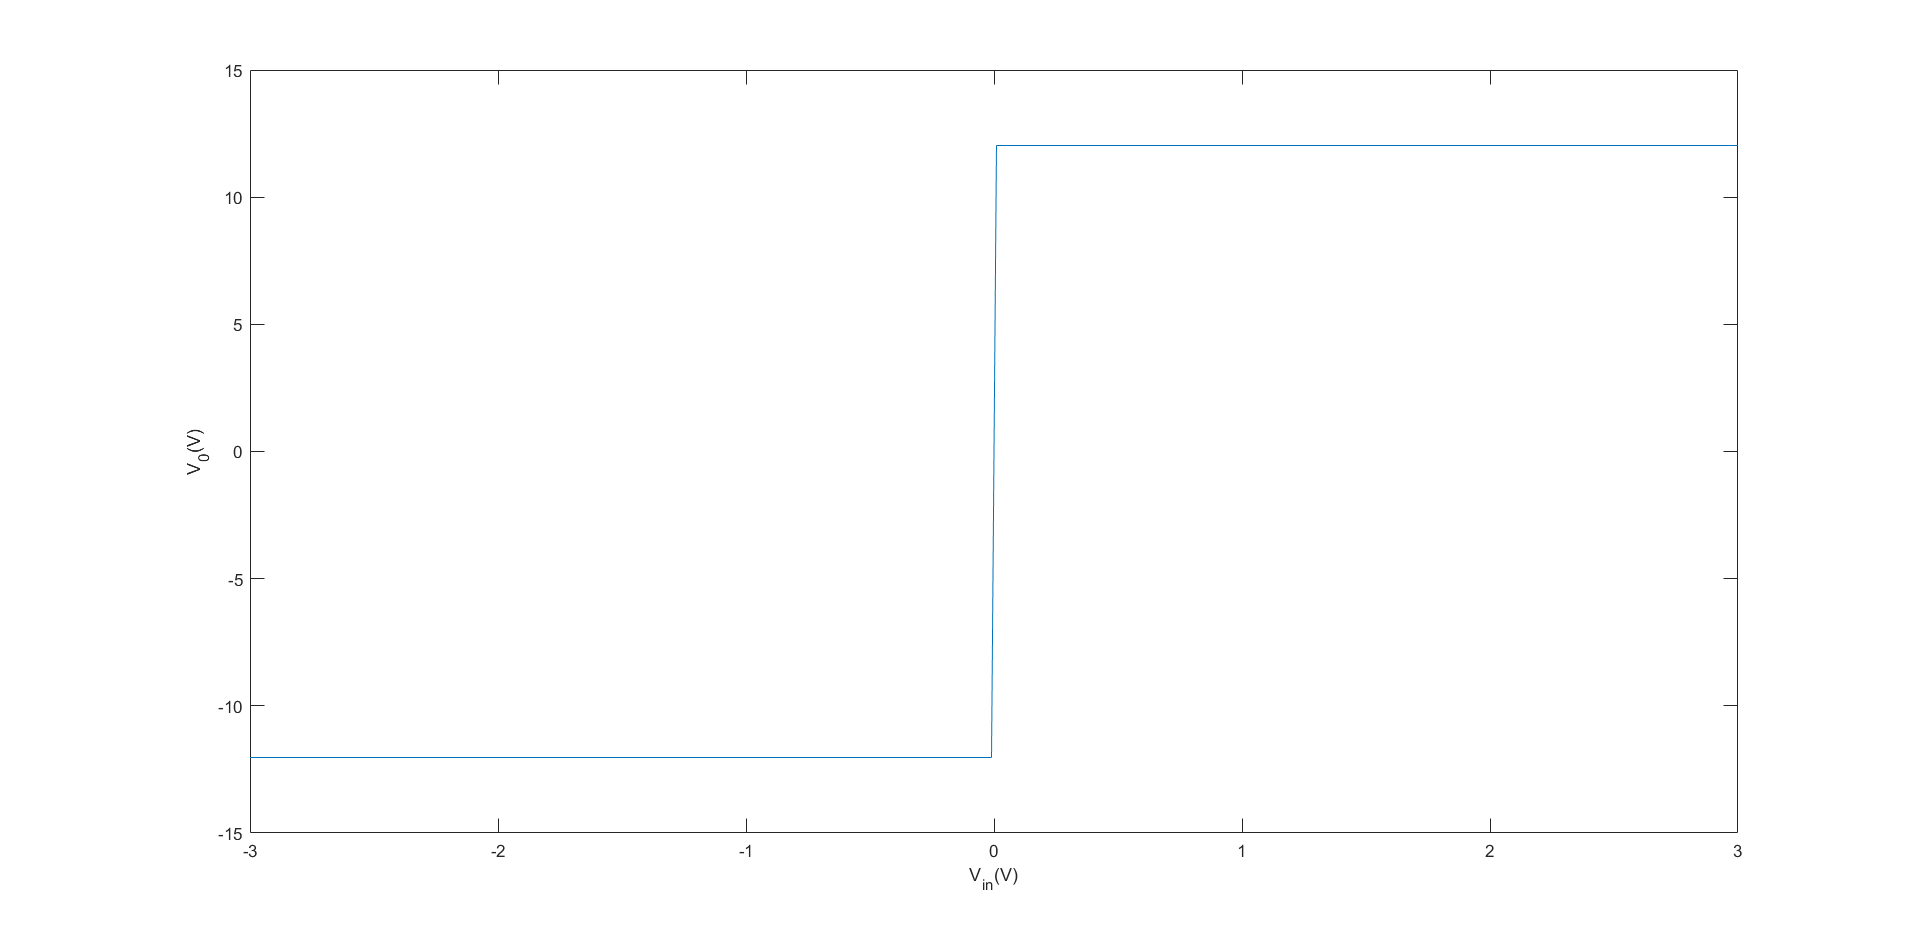
\includegraphics[width=1\textwidth]{3a_vs_vin.png}
   \caption{\(V_0\) vs \(V{in}\)}
\end{figure}

\begin{figure}[H]
	\centering
   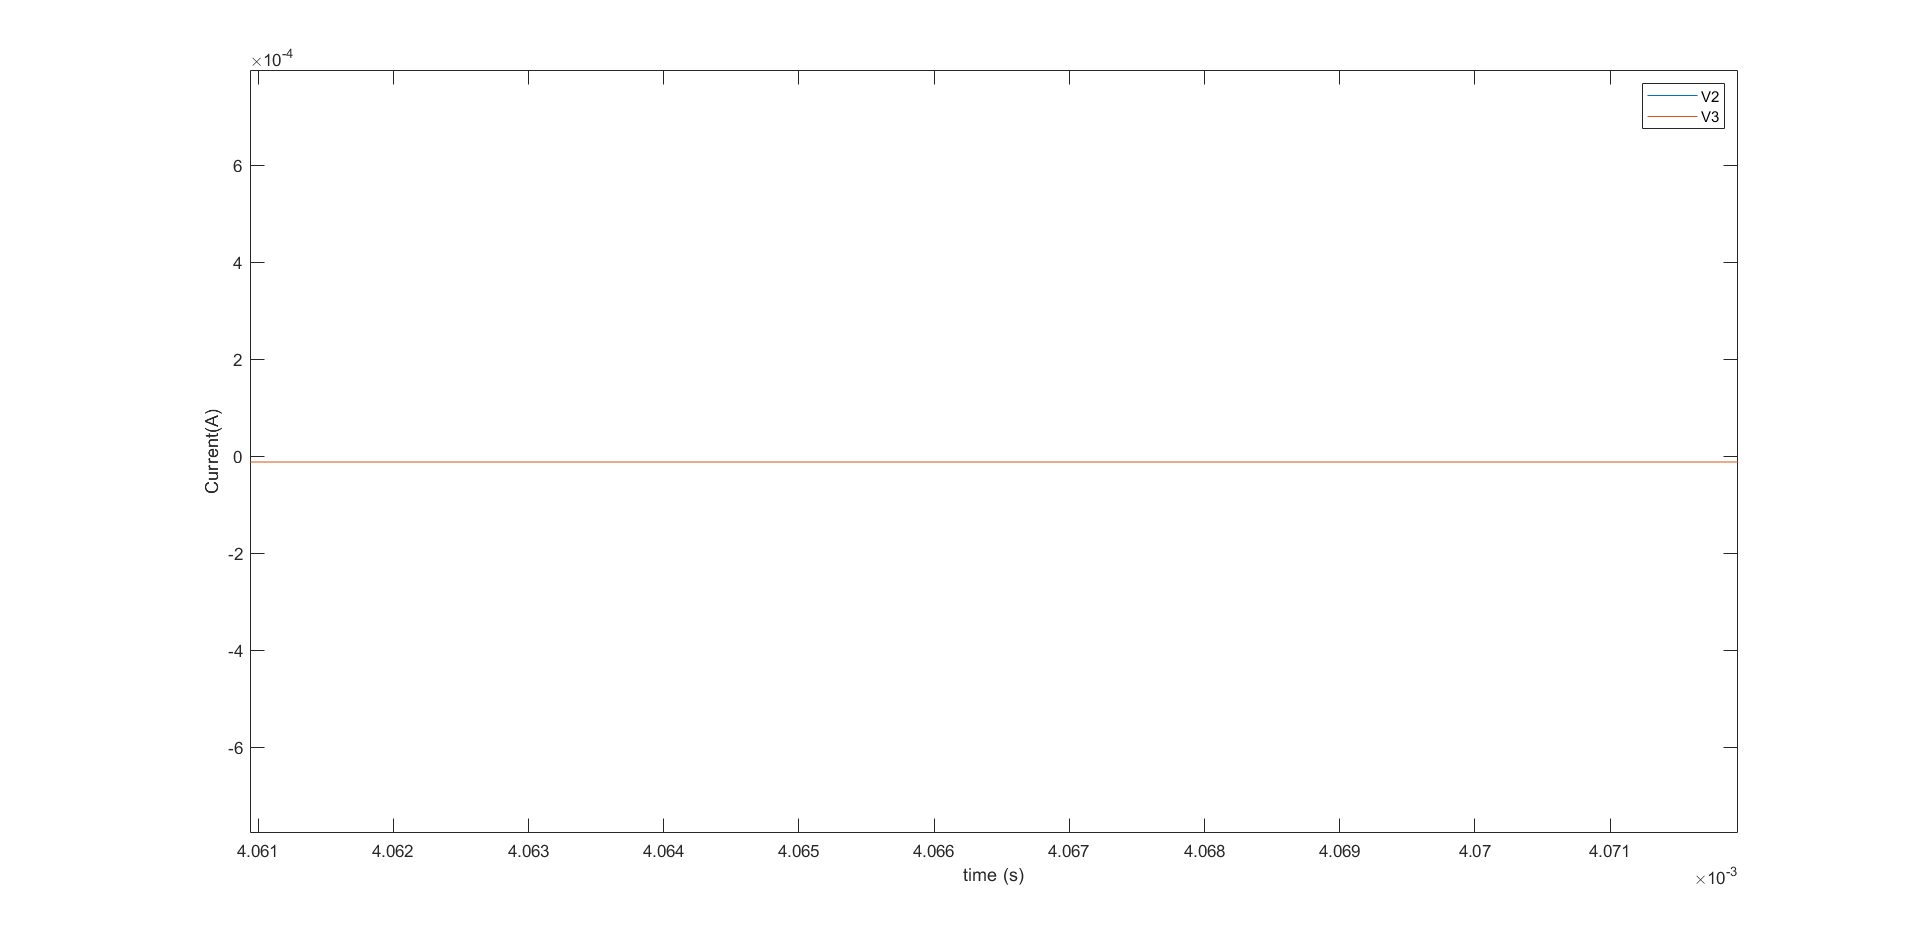
\includegraphics[width=1\textwidth]{3a_i.png}
   \caption{\(i\) vs t}
\end{figure}

\subsection{b)}
Buffer circuit is constructed in LTSpice environment. The schematic is given in the Figure 8.
\begin{figure}[H]
	\centering
   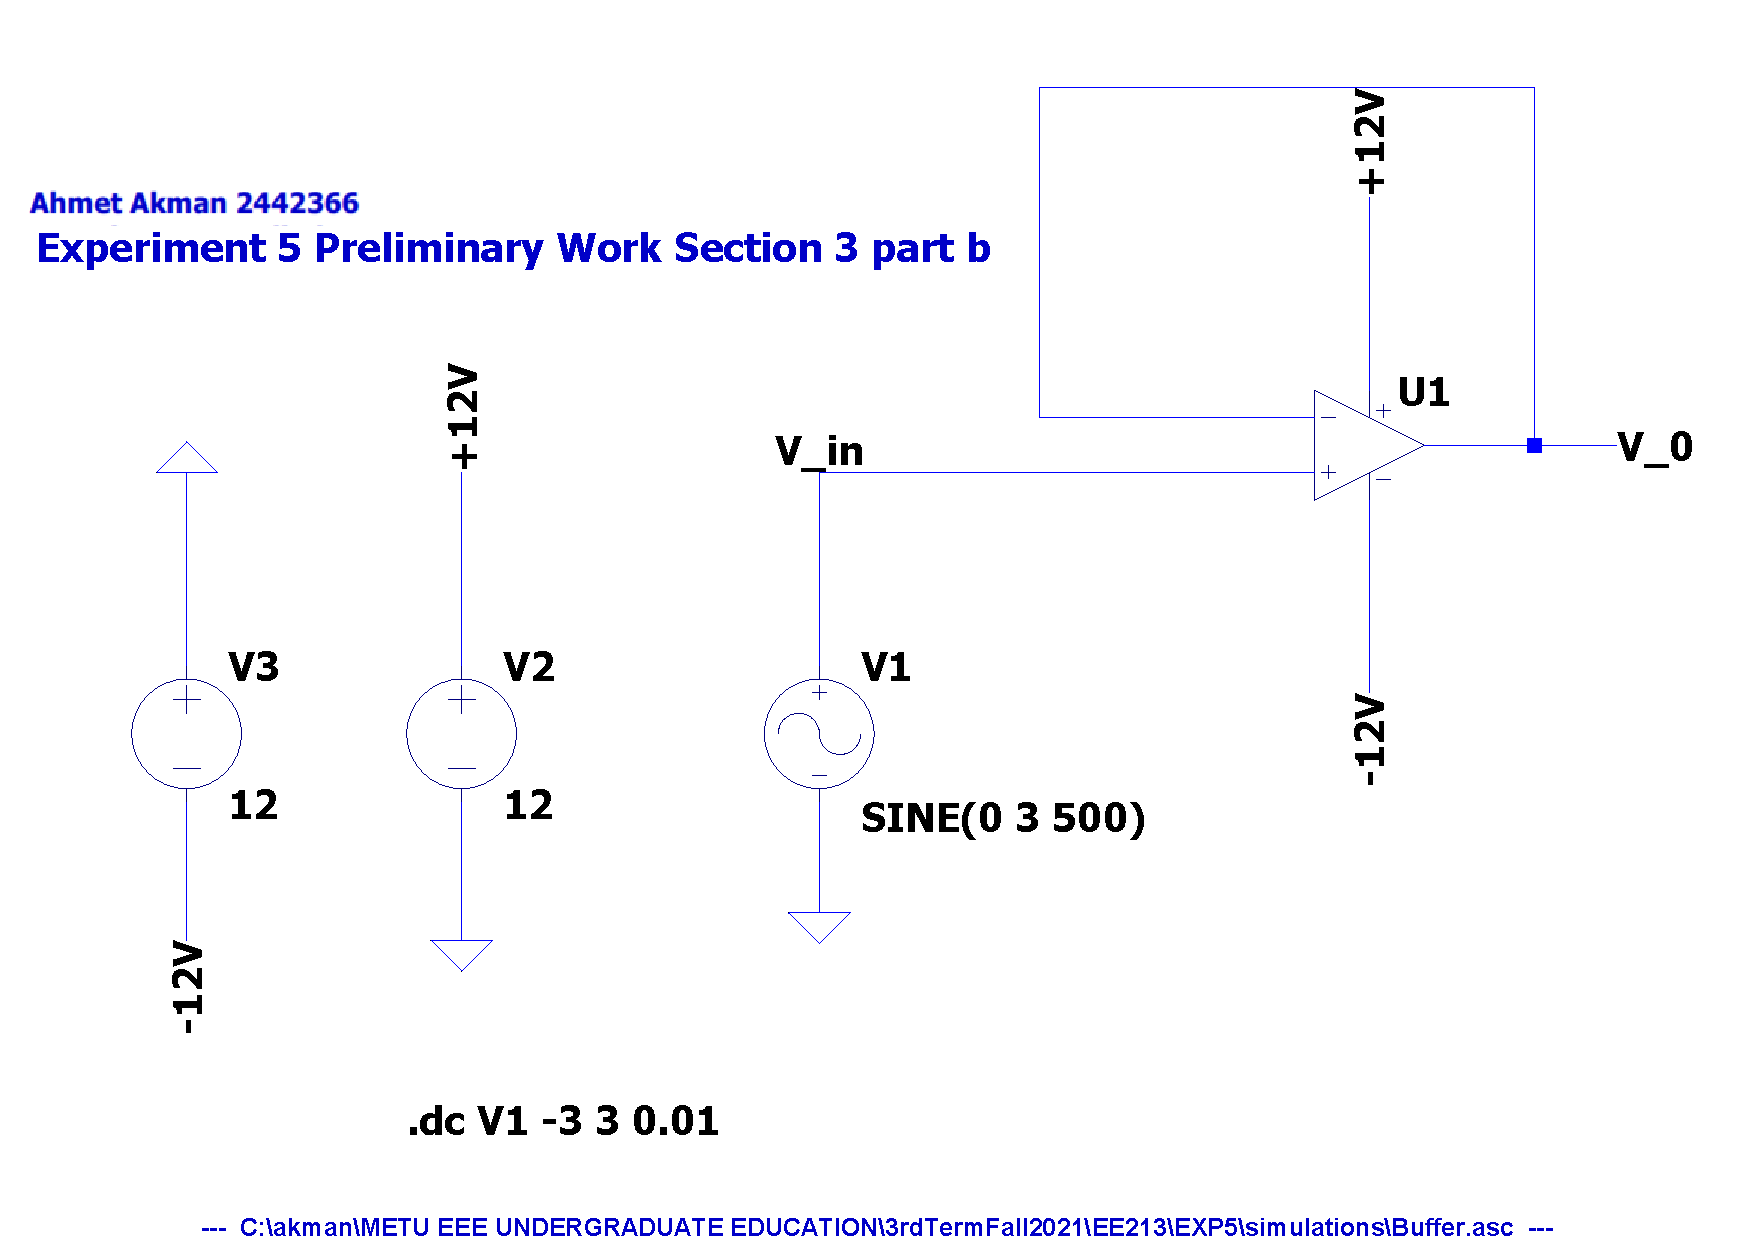
\includegraphics[width=0.8\textwidth]{Buffer_SCH.pdf}
   \caption{Circuit schematic for the buffer.}
\end{figure} 
Then plots given in Figures 9 , 10 and 11 are obtained.
\begin{figure}[H]
	\centering
   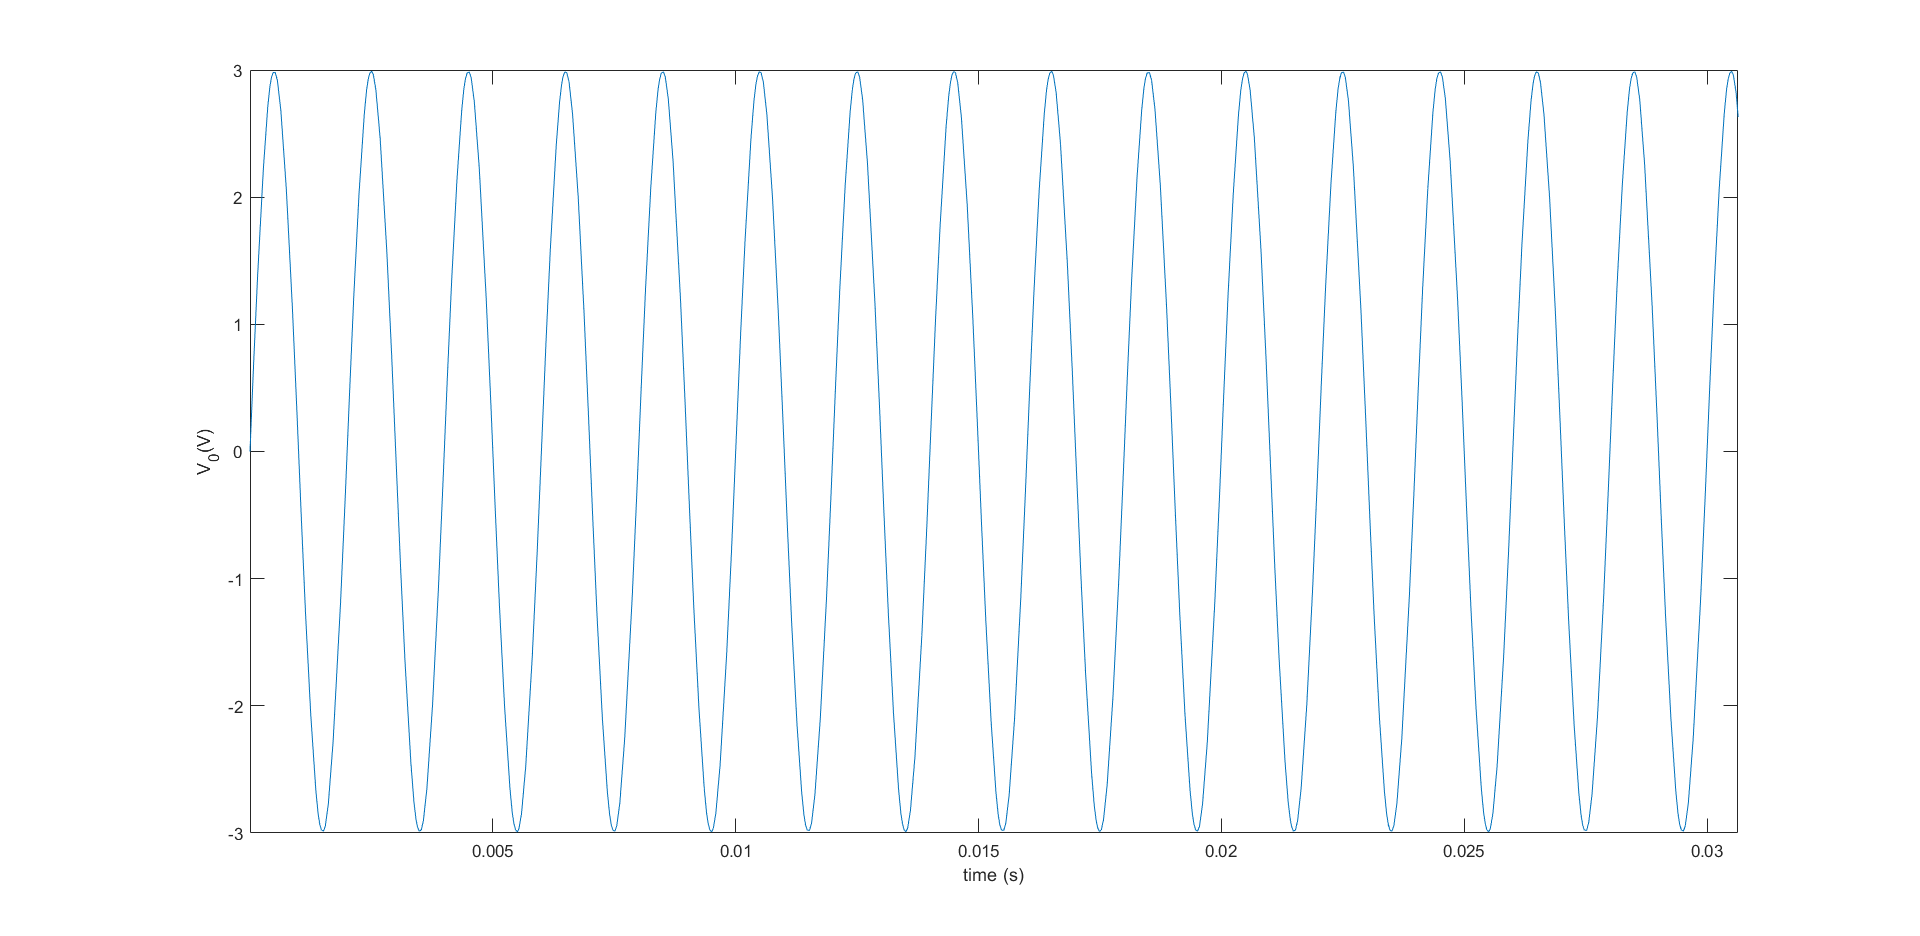
\includegraphics[width=1\textwidth]{3b_vs_t.png}
   \caption{\(V_0\) vs t}
\end{figure}

\begin{figure}[H]
	\centering
   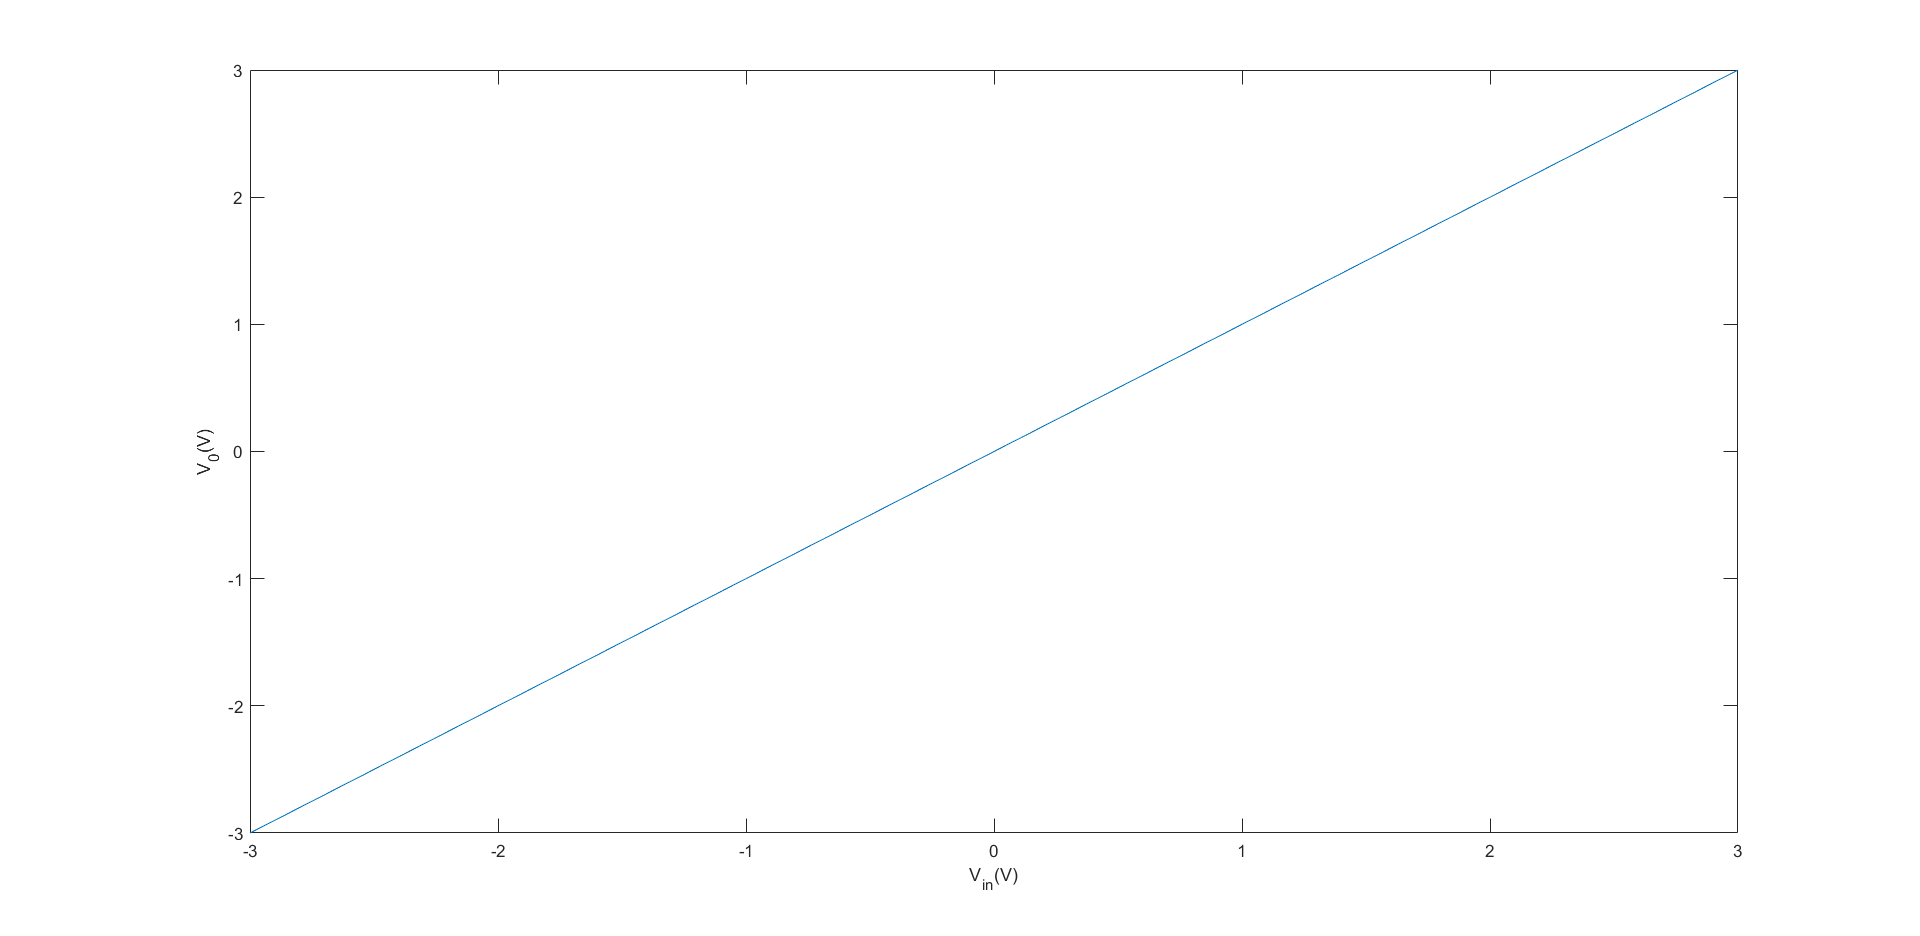
\includegraphics[width=1\textwidth]{3b_vs_vin.png}
   \caption{\(V_0\) vs \(V{in}\)}
\end{figure}

\begin{figure}[H]
	\centering
   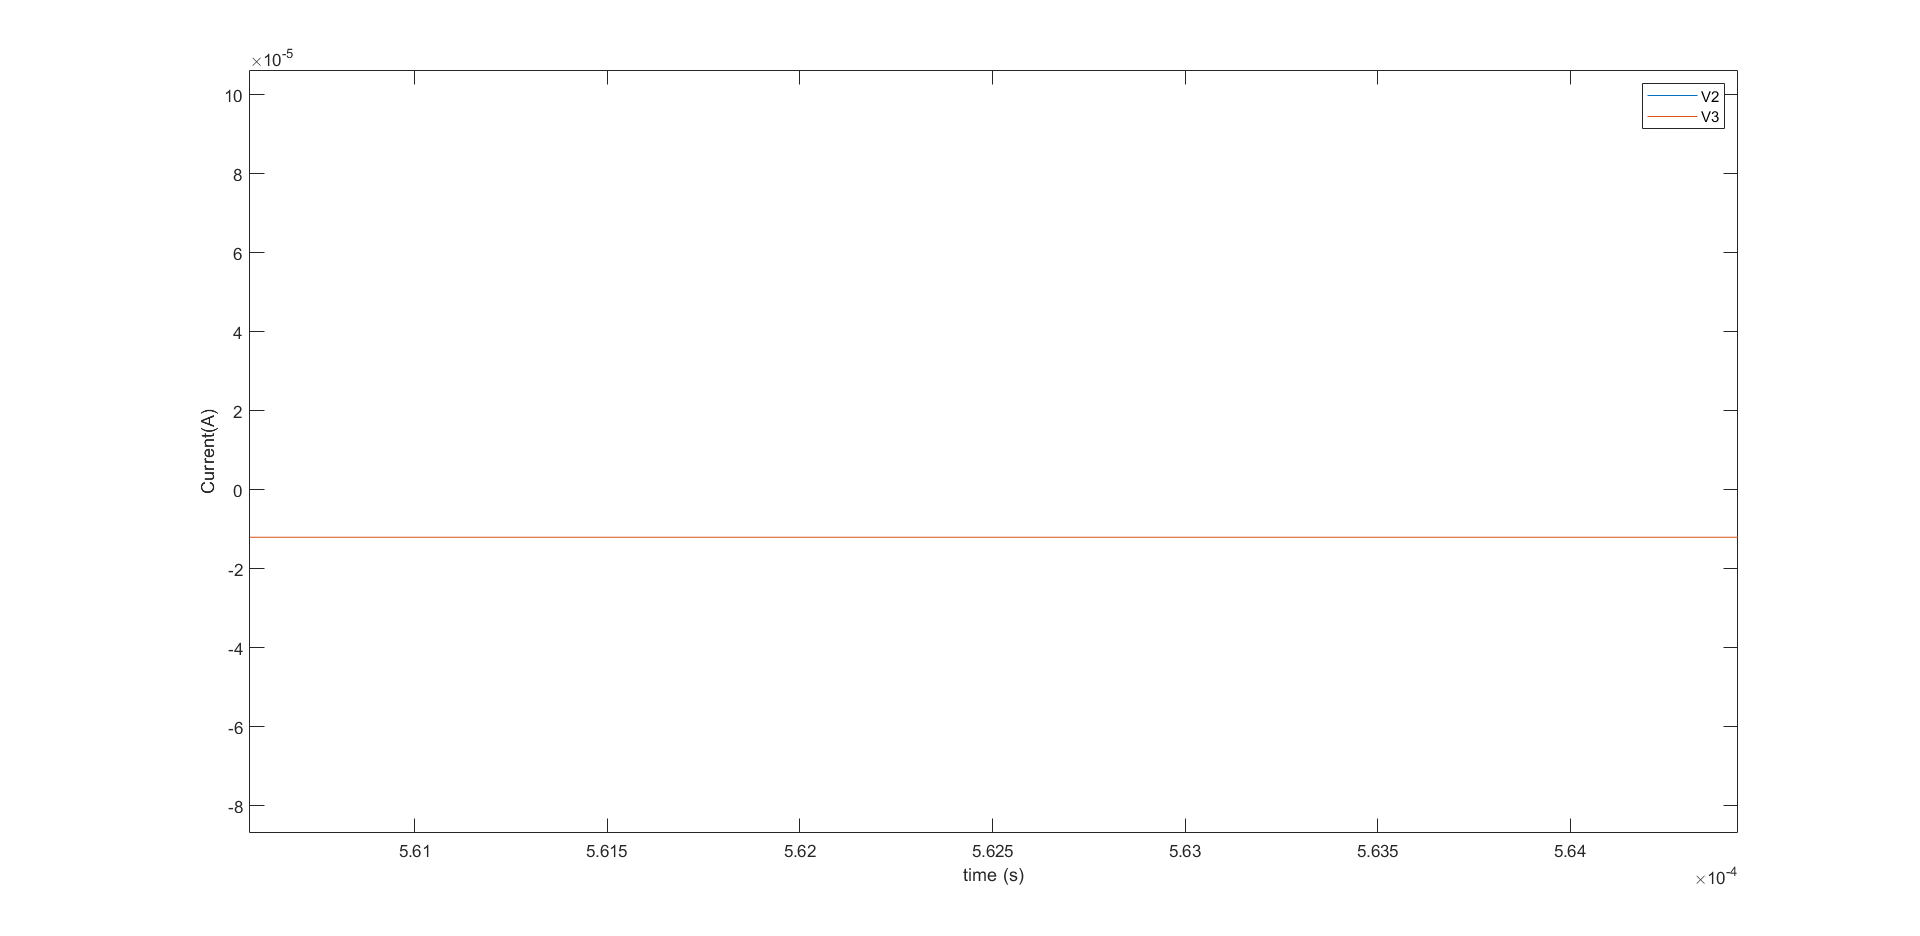
\includegraphics[width=0.8\textwidth]{3b_i.png}
   \caption{\(i\) vs t}
\end{figure}

\subsection{c)}
Inverting amplifier circuit is constructed in LTSpice environment. The schematic is given in the Figure 12.
\begin{figure}[H]
	\centering
   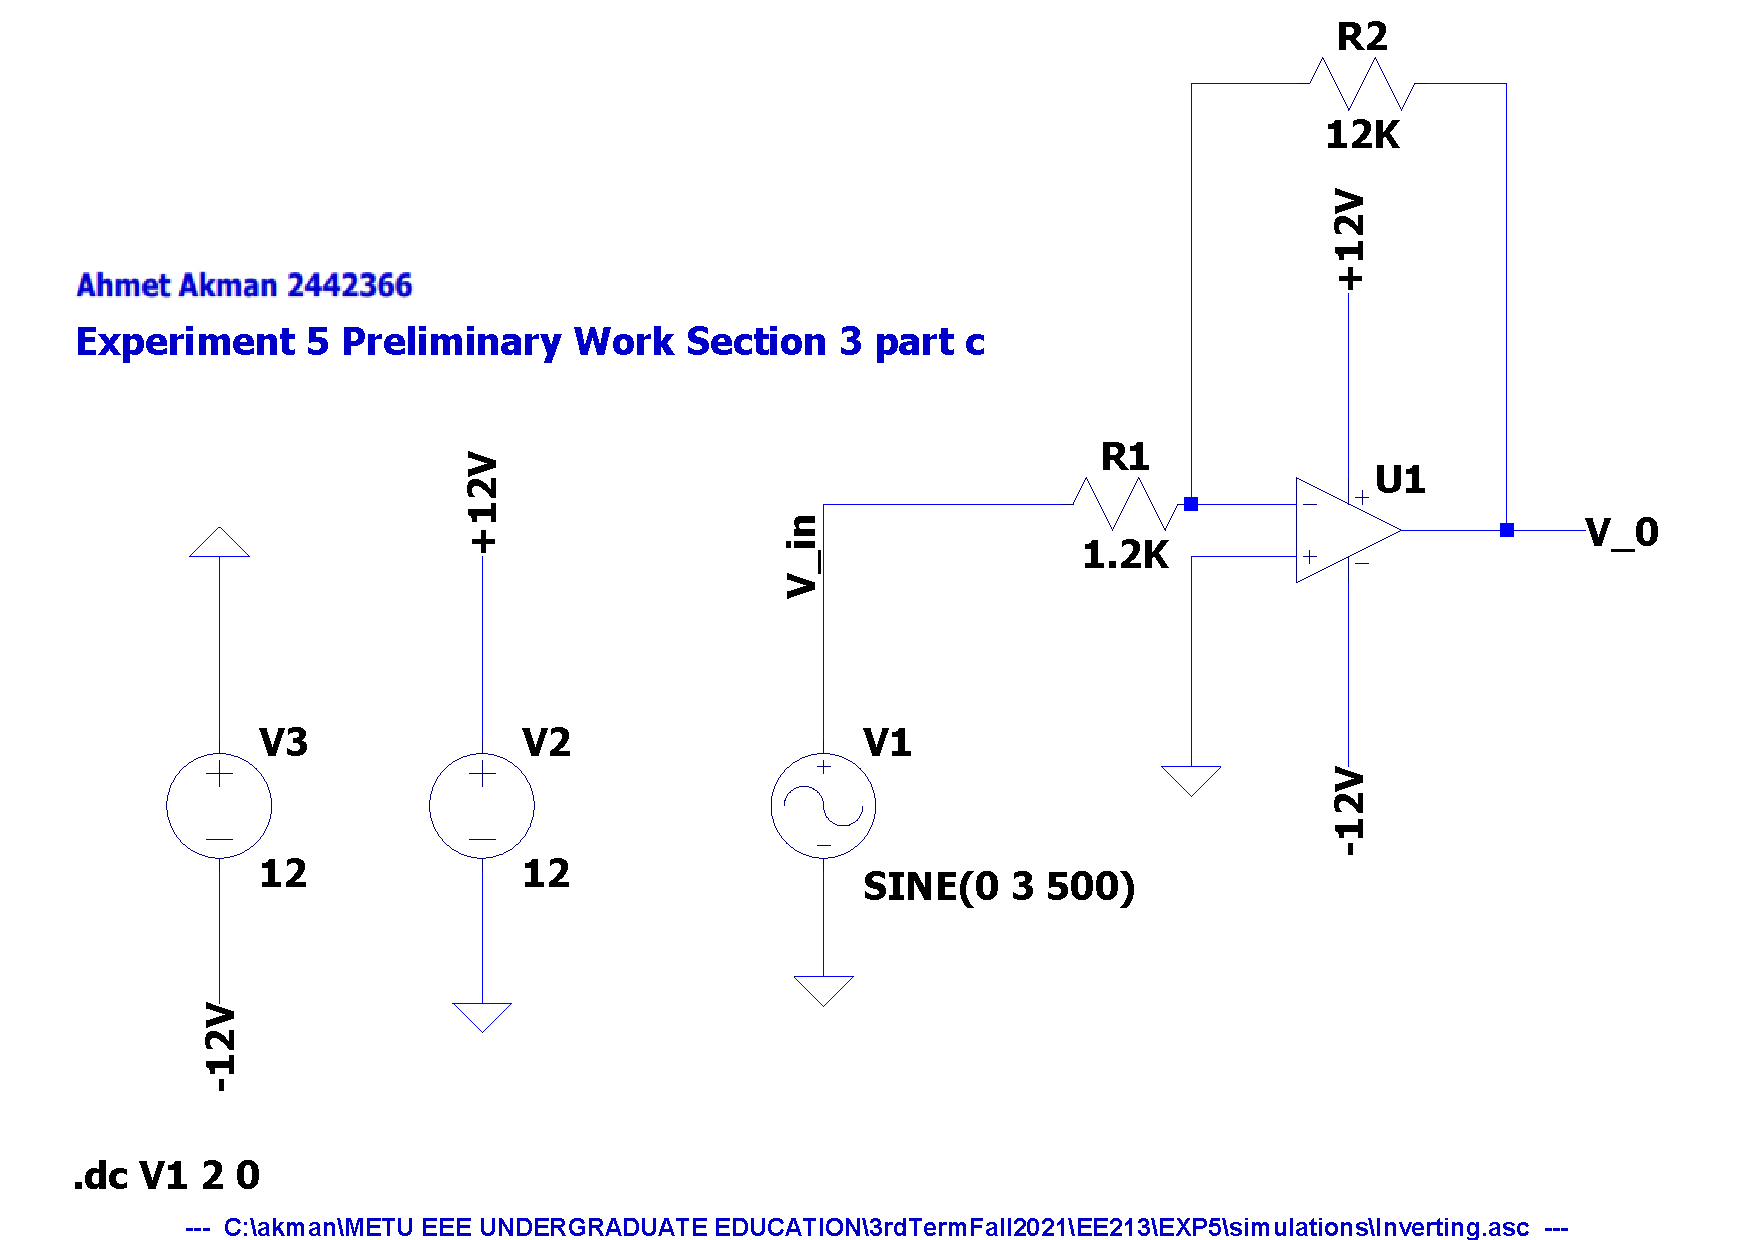
\includegraphics[width=1\textwidth]{Inverting_SCH.pdf}
   \caption{Circuit schematic for the inverting amplifier.}
\end{figure} 
Then plots given in Figures 13,14 and 15 are obtained.
\begin{figure}[H]
	\centering
   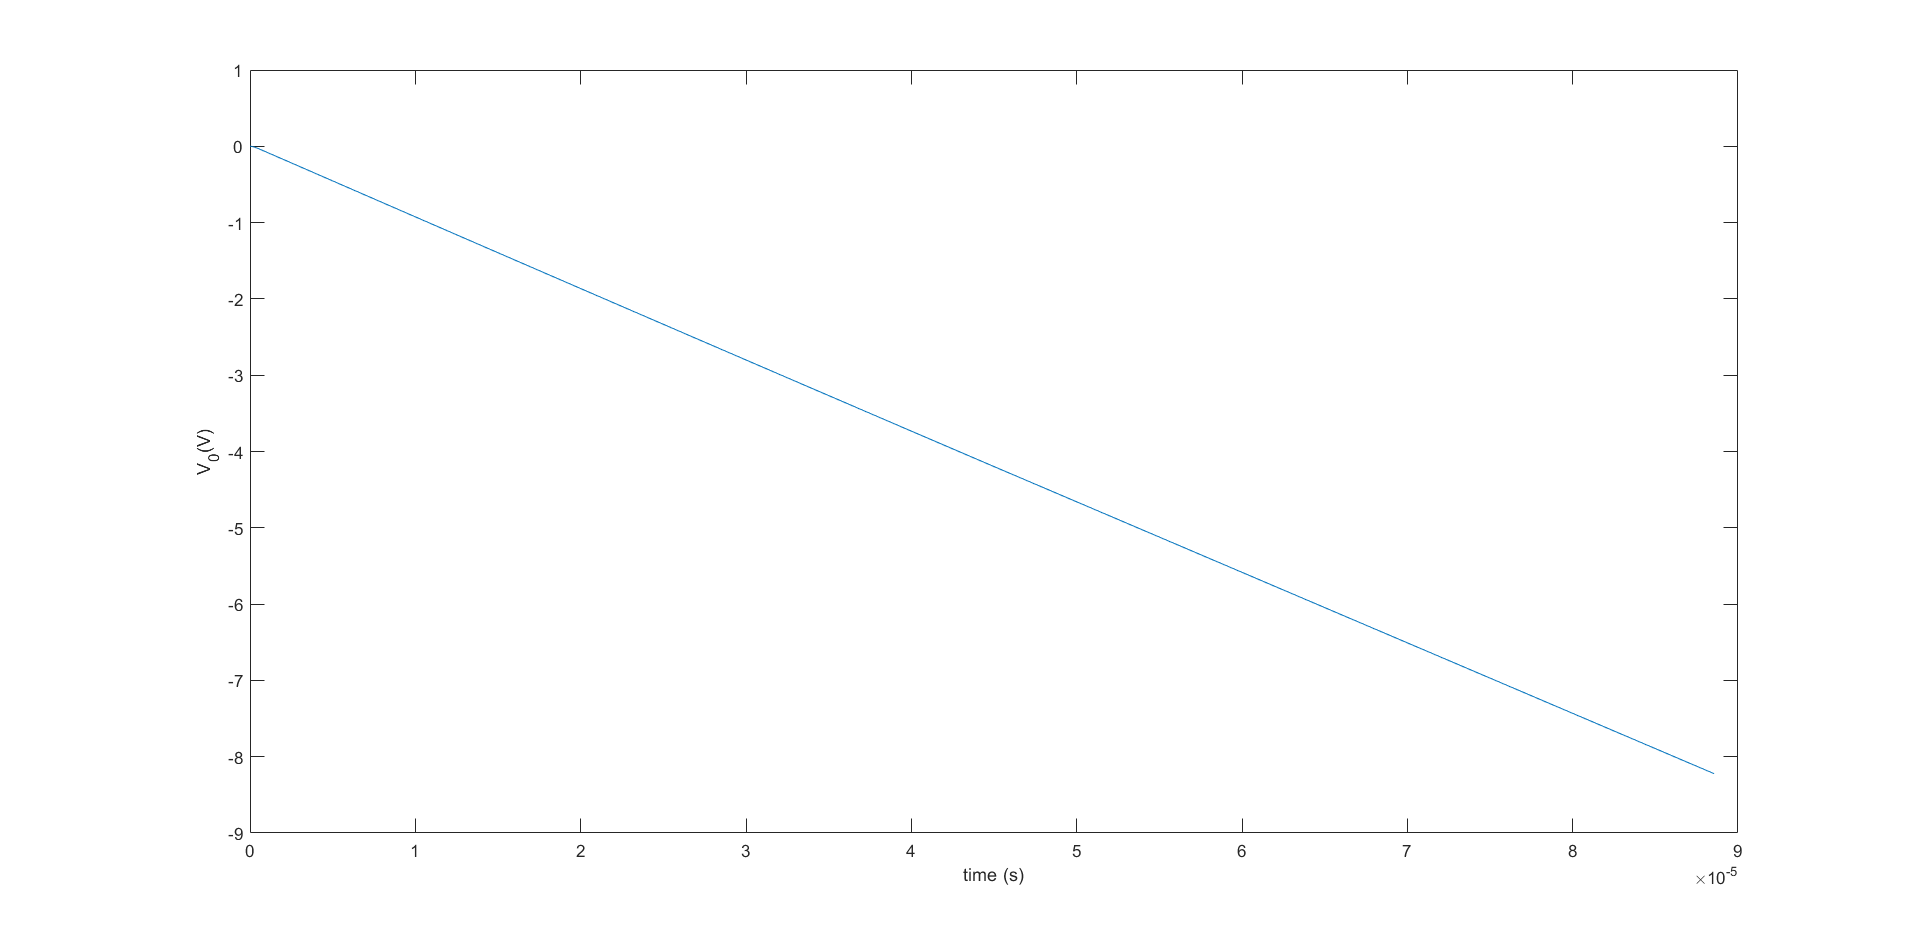
\includegraphics[width=1\textwidth]{3c_vs_t.png}
   \caption{\(V_0\) vs t}
\end{figure}

\begin{figure}[H]
	\centering
   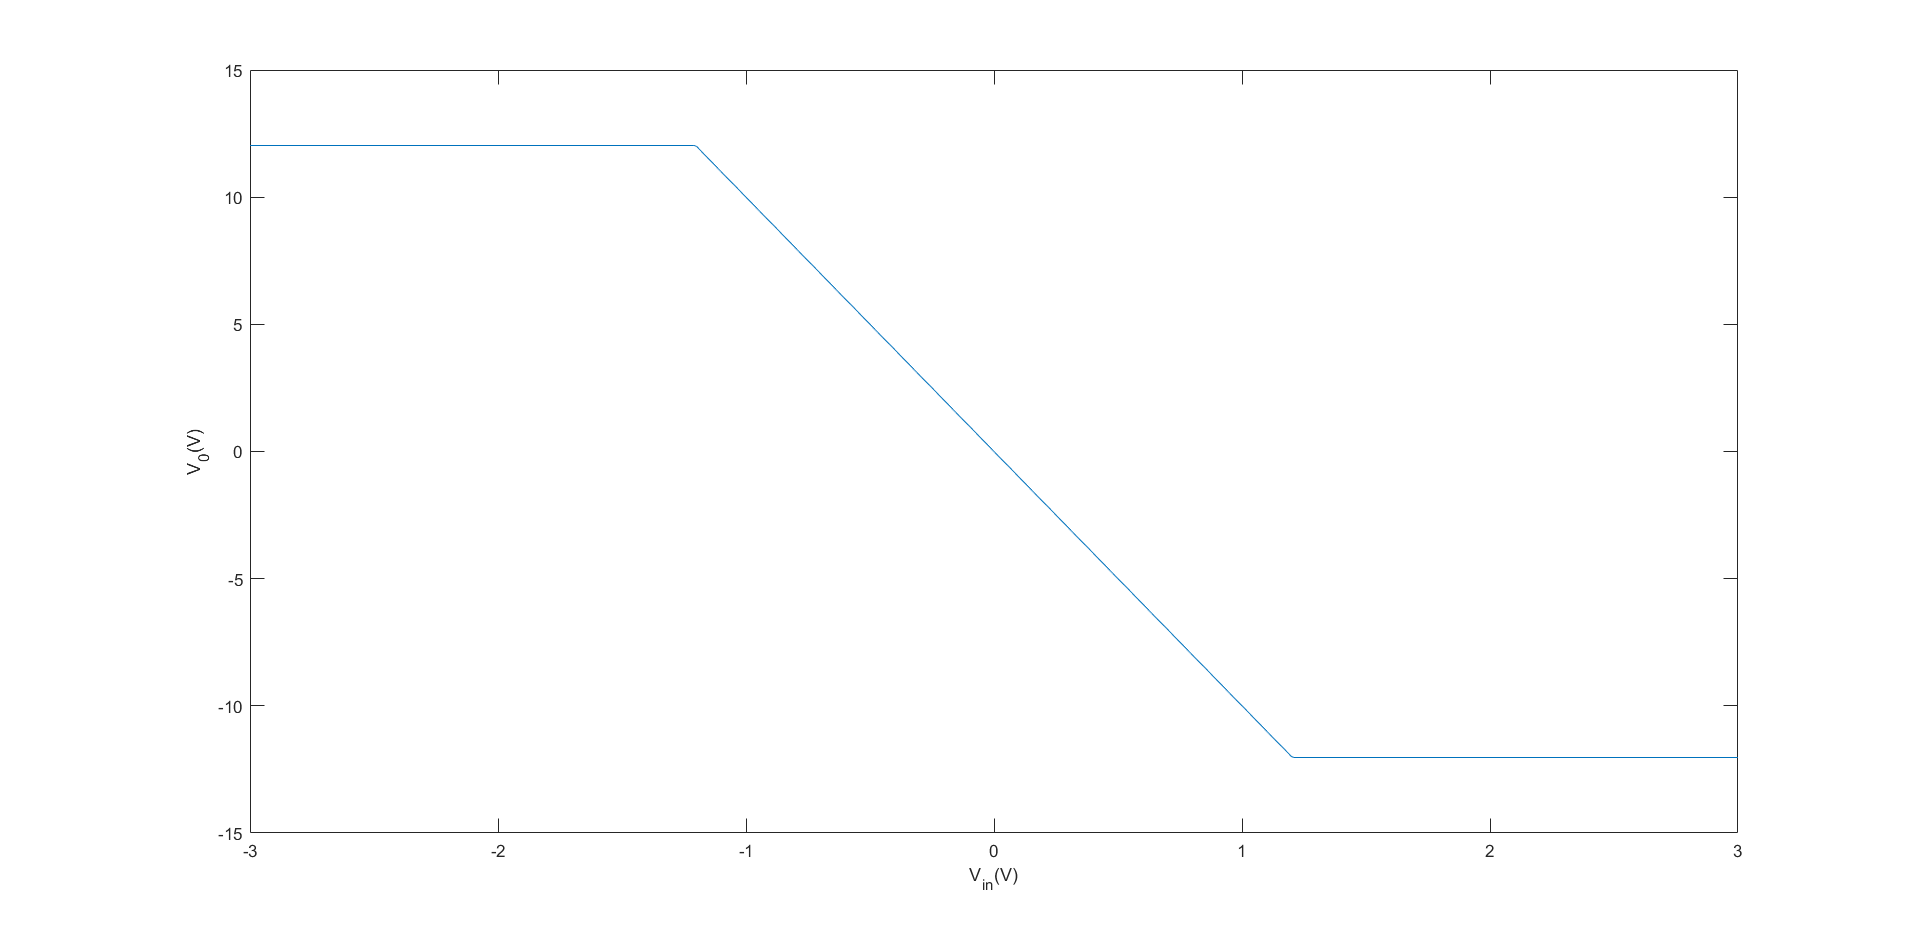
\includegraphics[width=1\textwidth]{3c_vs_vin.png}
   \caption{\(V_0\) vs \(V{in}\)}
\end{figure}

\begin{figure}[H]
	\centering
   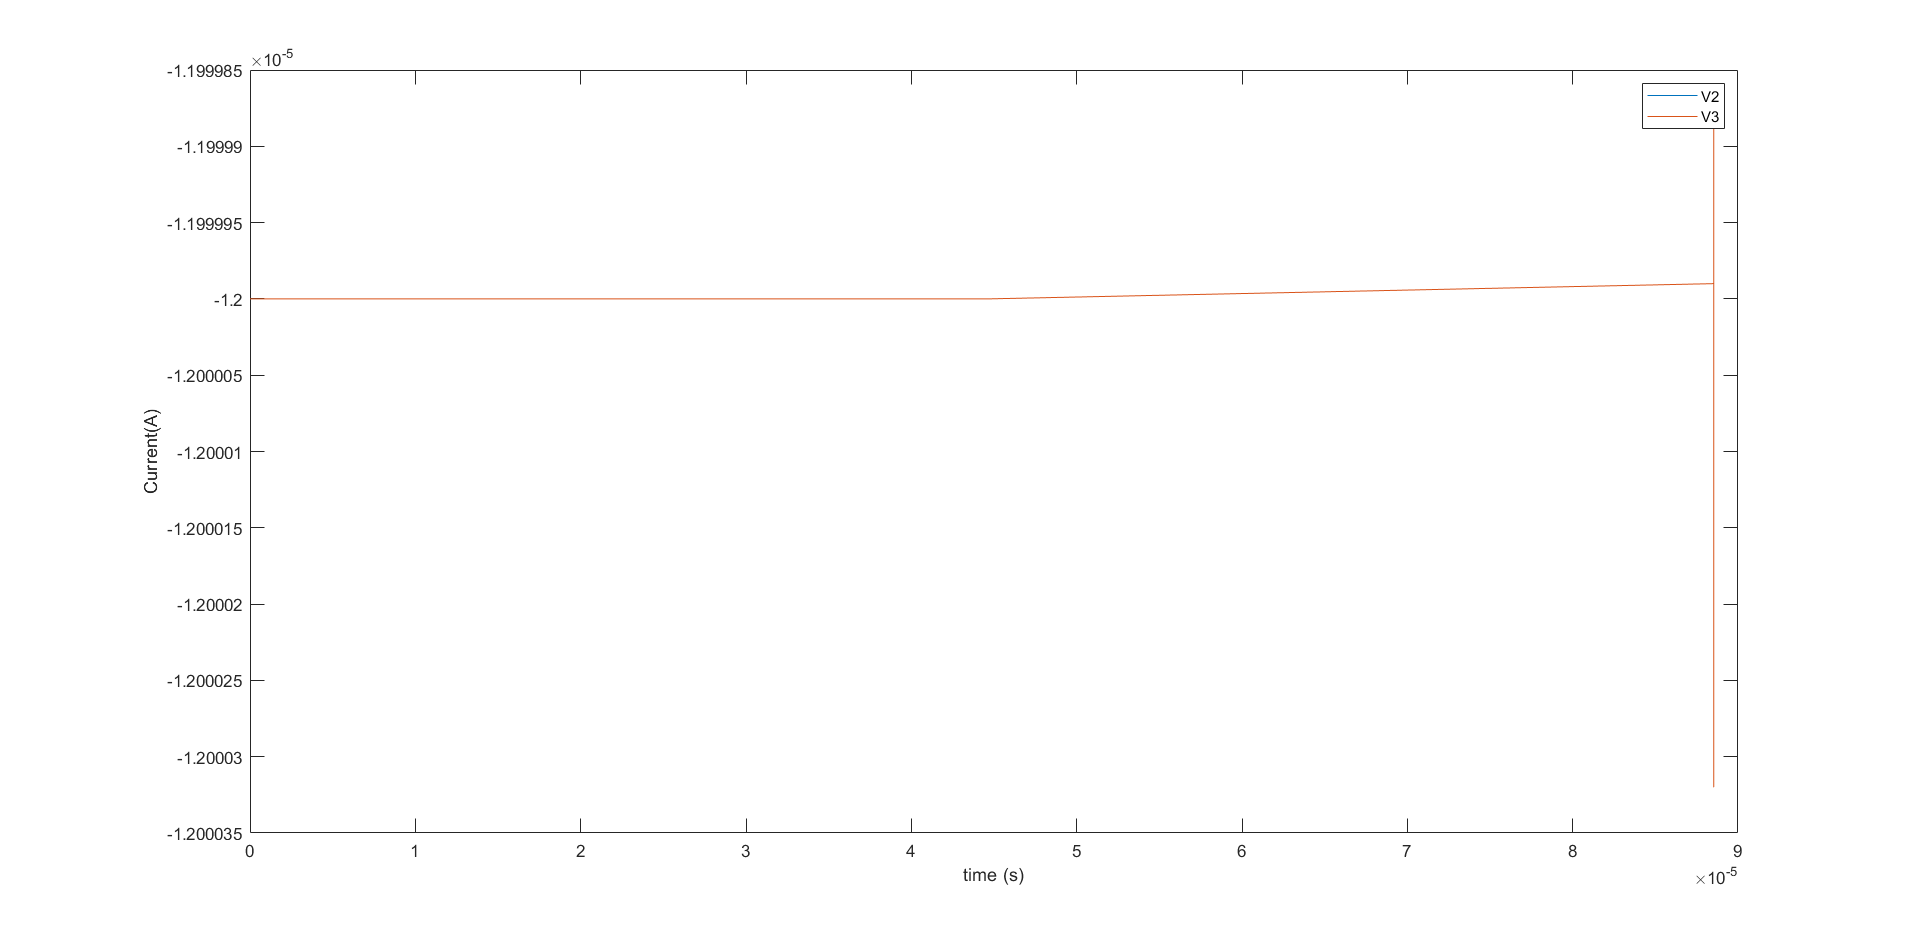
\includegraphics[width=1\textwidth]{3c_i.png}
   \caption{\(i\) vs t}
\end{figure}

\subsection{d)}
Non-inverting amplifier circuit is constructed in LTSpice environment. The schematic is given in the Figure 16.
\begin{figure}[H]
	\centering
   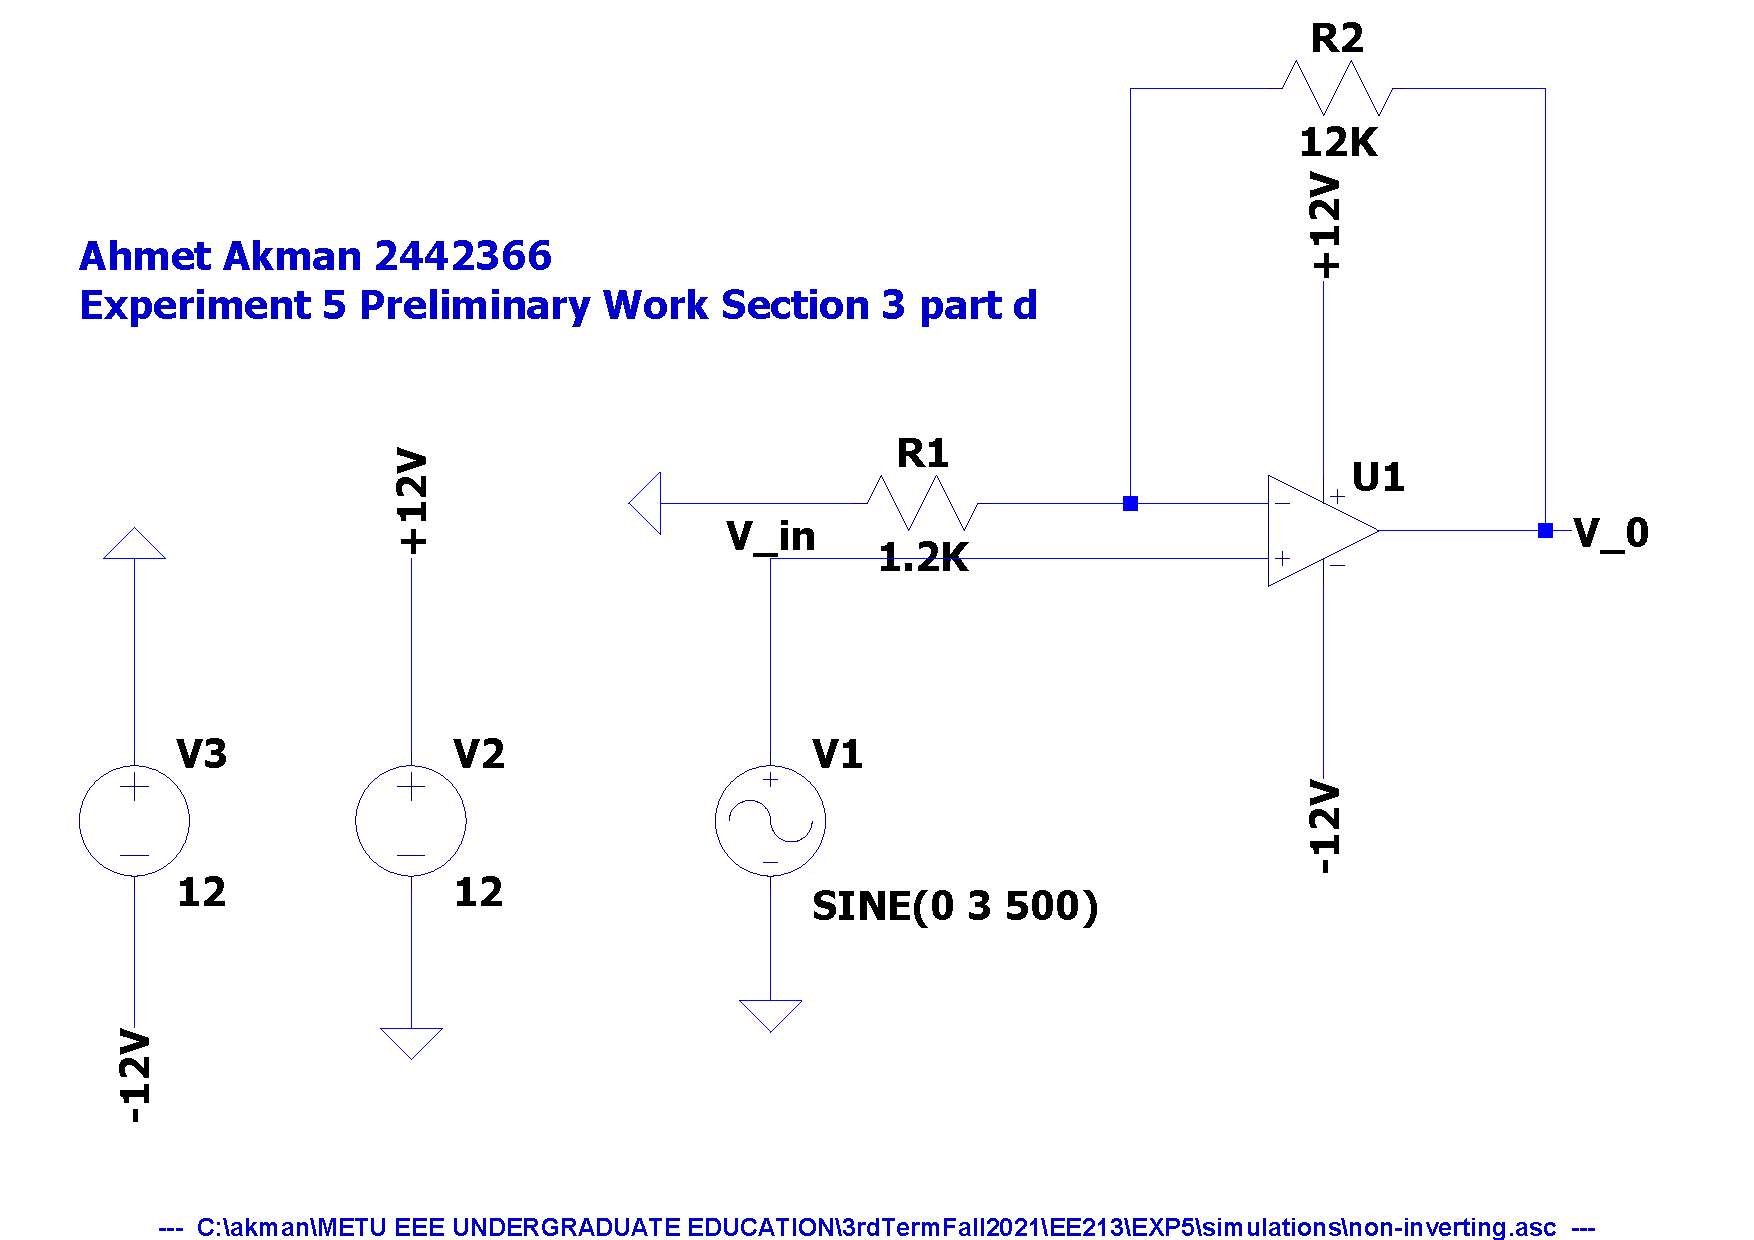
\includegraphics[width=0.8\textwidth]{non-inverting_SCH.pdf}
   \caption{Circuit schematic for the basic comparator.}
\end{figure} 
Then plots given in Figures 17,18 and 19 are obtained.
\begin{figure}[H]
	\centering
   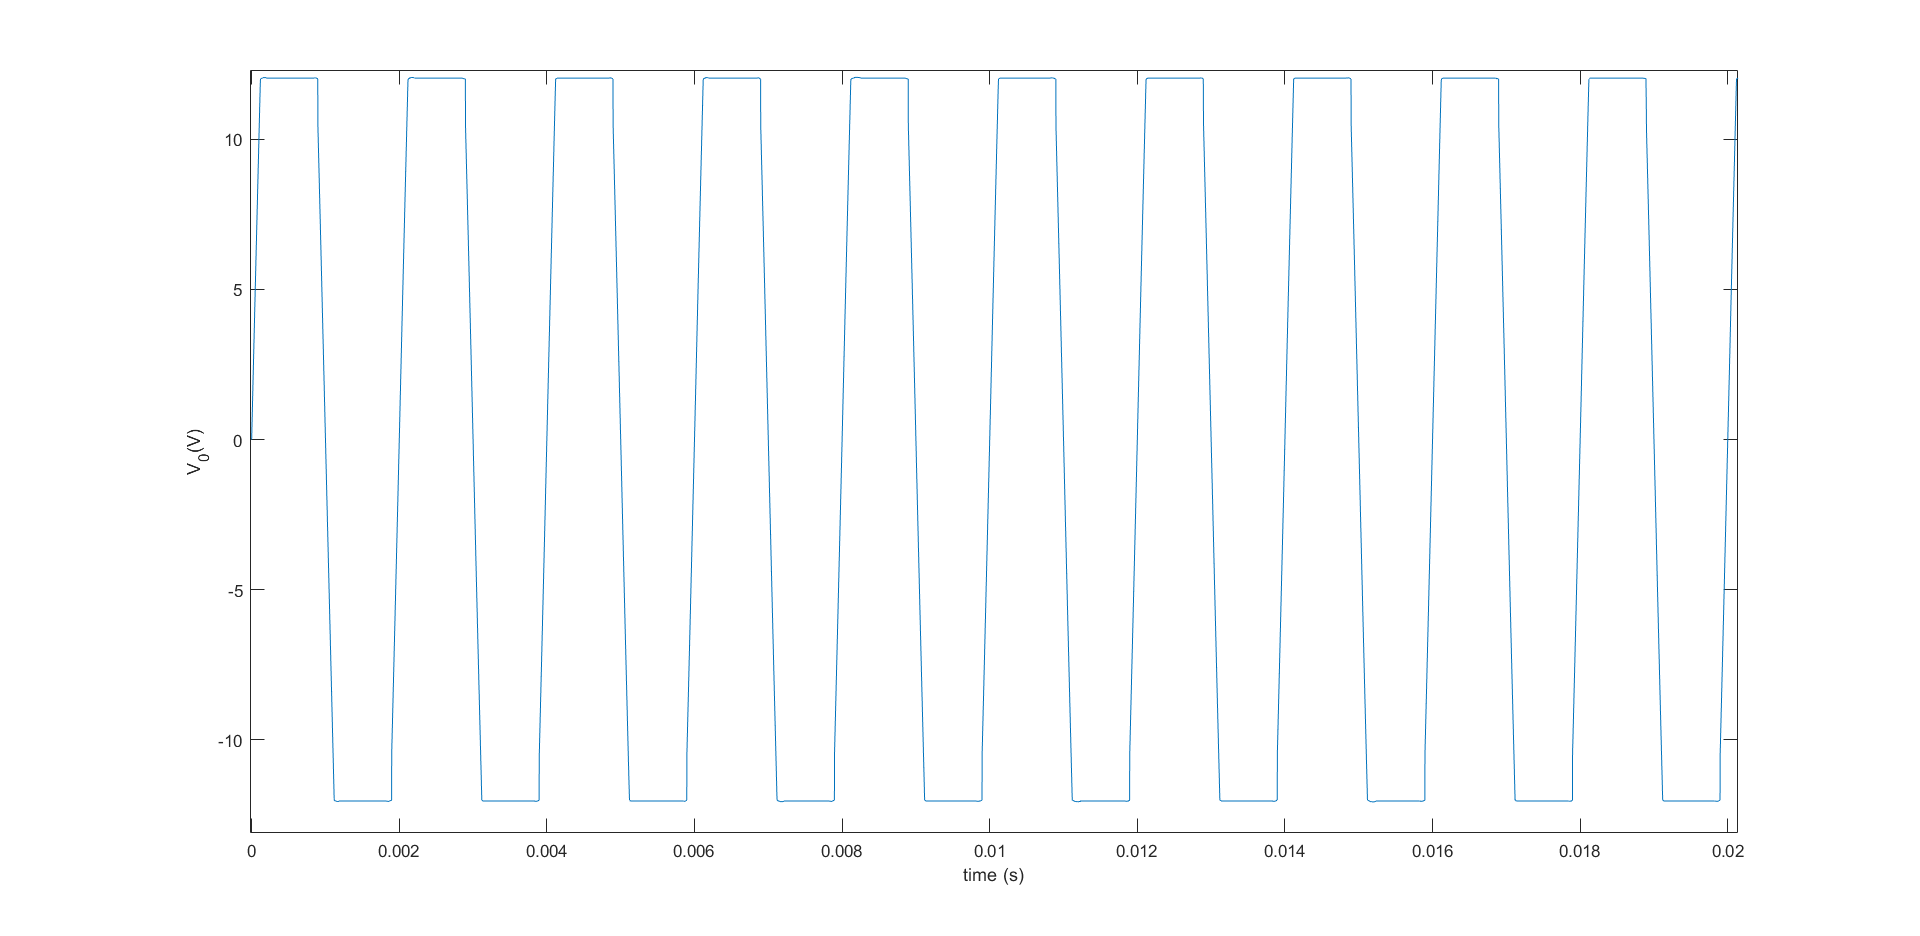
\includegraphics[width=1\textwidth]{3d_vs_t.png}
   \caption{\(V_0\) vs t}
\end{figure}

\begin{figure}[H]
	\centering
   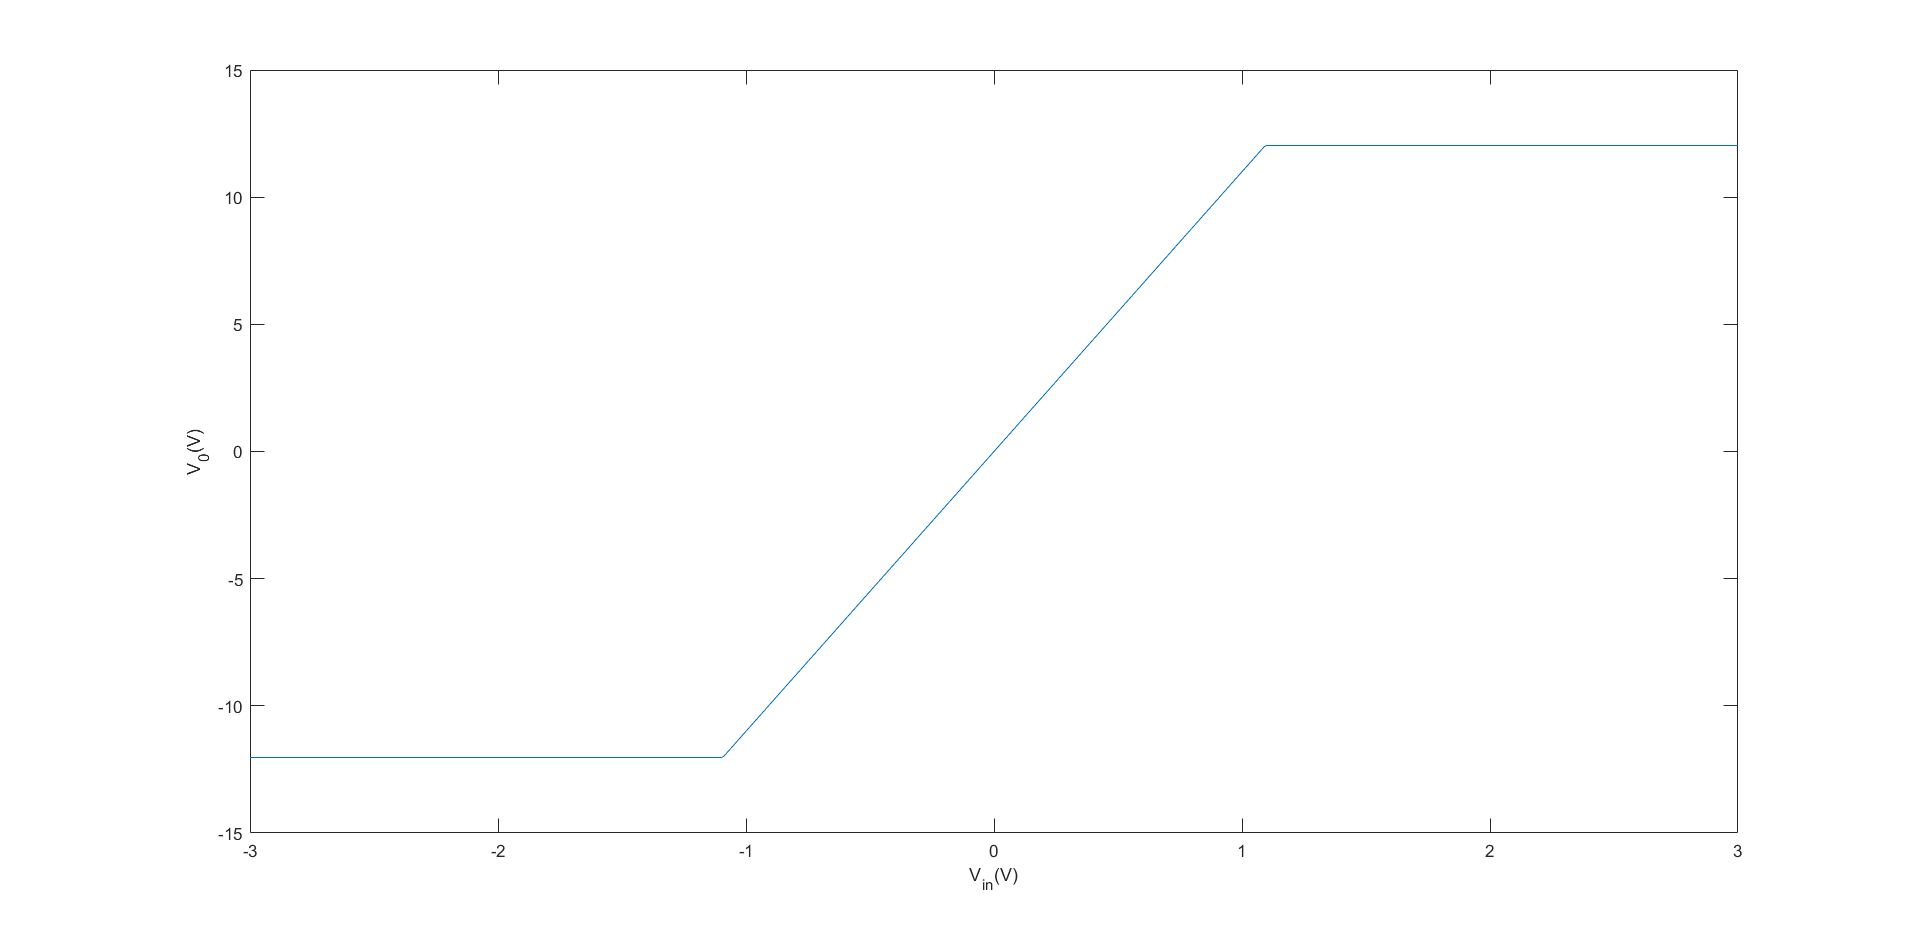
\includegraphics[width=1\textwidth]{3d_vs_vin.png}
   \caption{\(V_0\) vs \(V{in}\)}
\end{figure}

\begin{figure}[H]
	\centering
   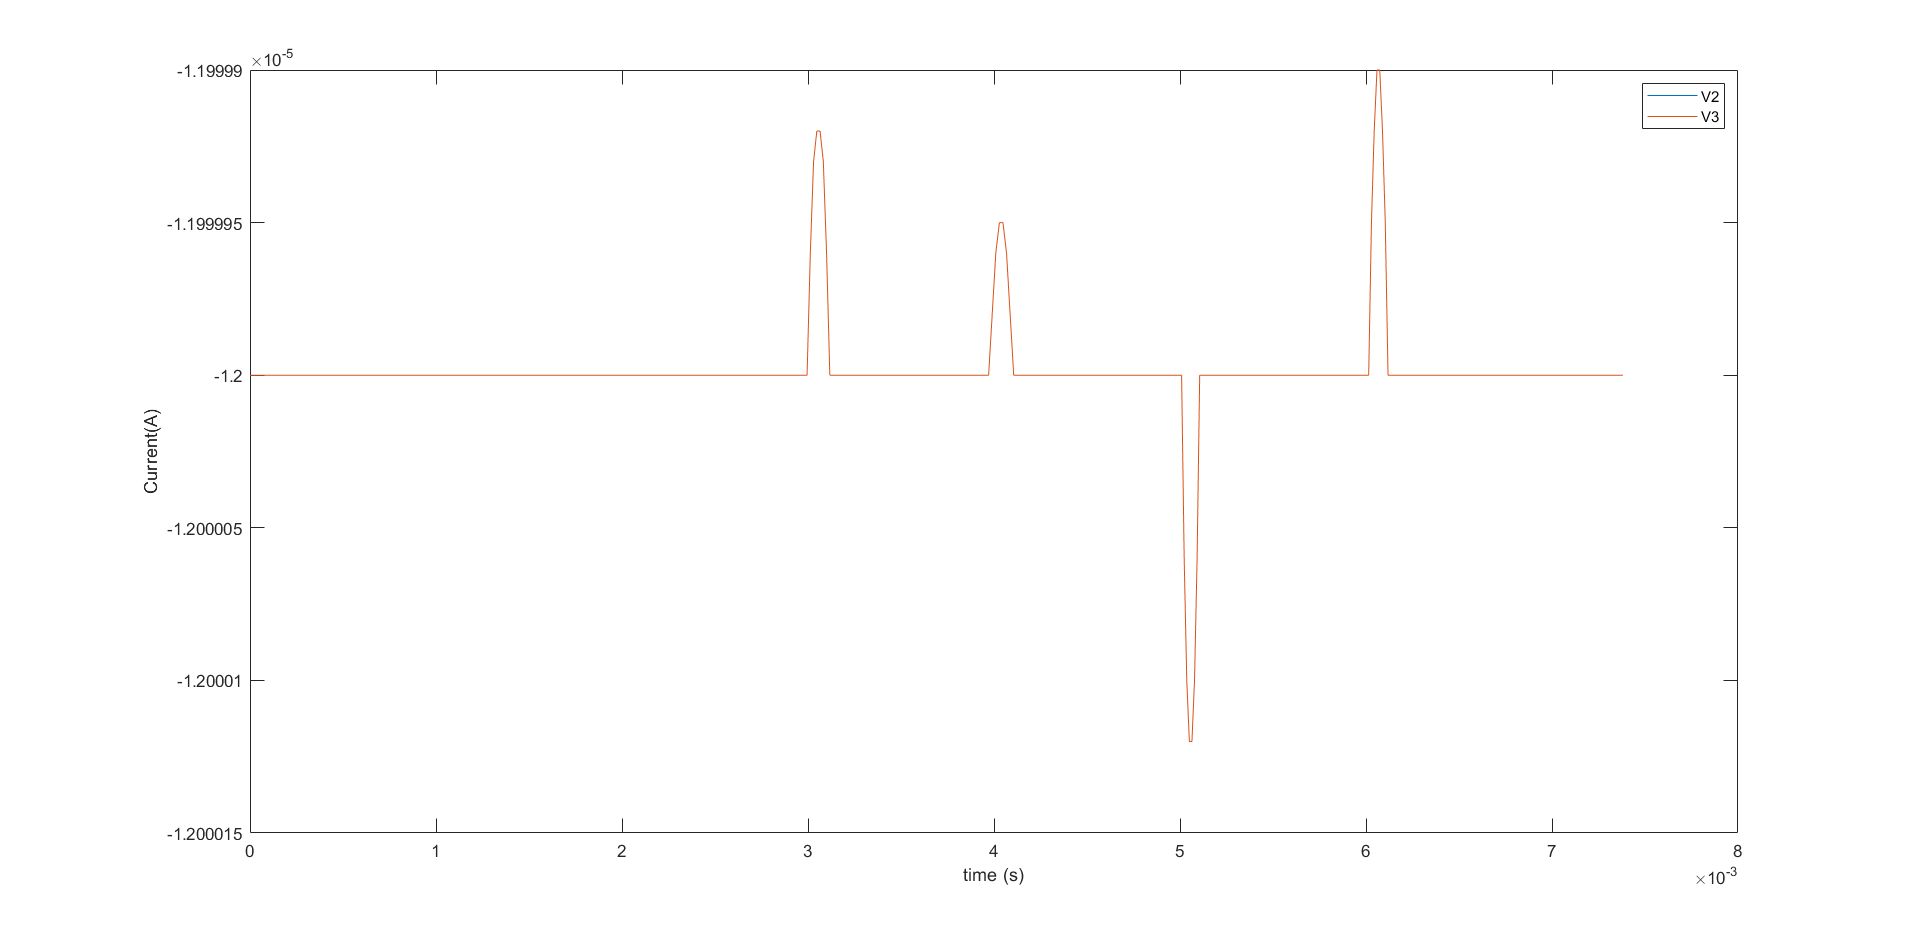
\includegraphics[width=1\textwidth]{3d_i.png}
   \caption{\(i\) vs t}
\end{figure}

\section{Step 4}
In this step following 2 op-amp circuits are constructed in the LTSpice environment and simulated. \(V_{a}\) is taken as \(4sin(1000\pi)\) Volts. \(V_{b}\) is taken as \(2sin(1000\pi)\) Volts. Then data are fetched from LTSpice and plotted in MATLAB.

\subsection{a)}
Summing amplifier circuit is constructed in LTSpice environment. The schematic is given in the Figure 20.
\begin{figure}[H]
	\centering
   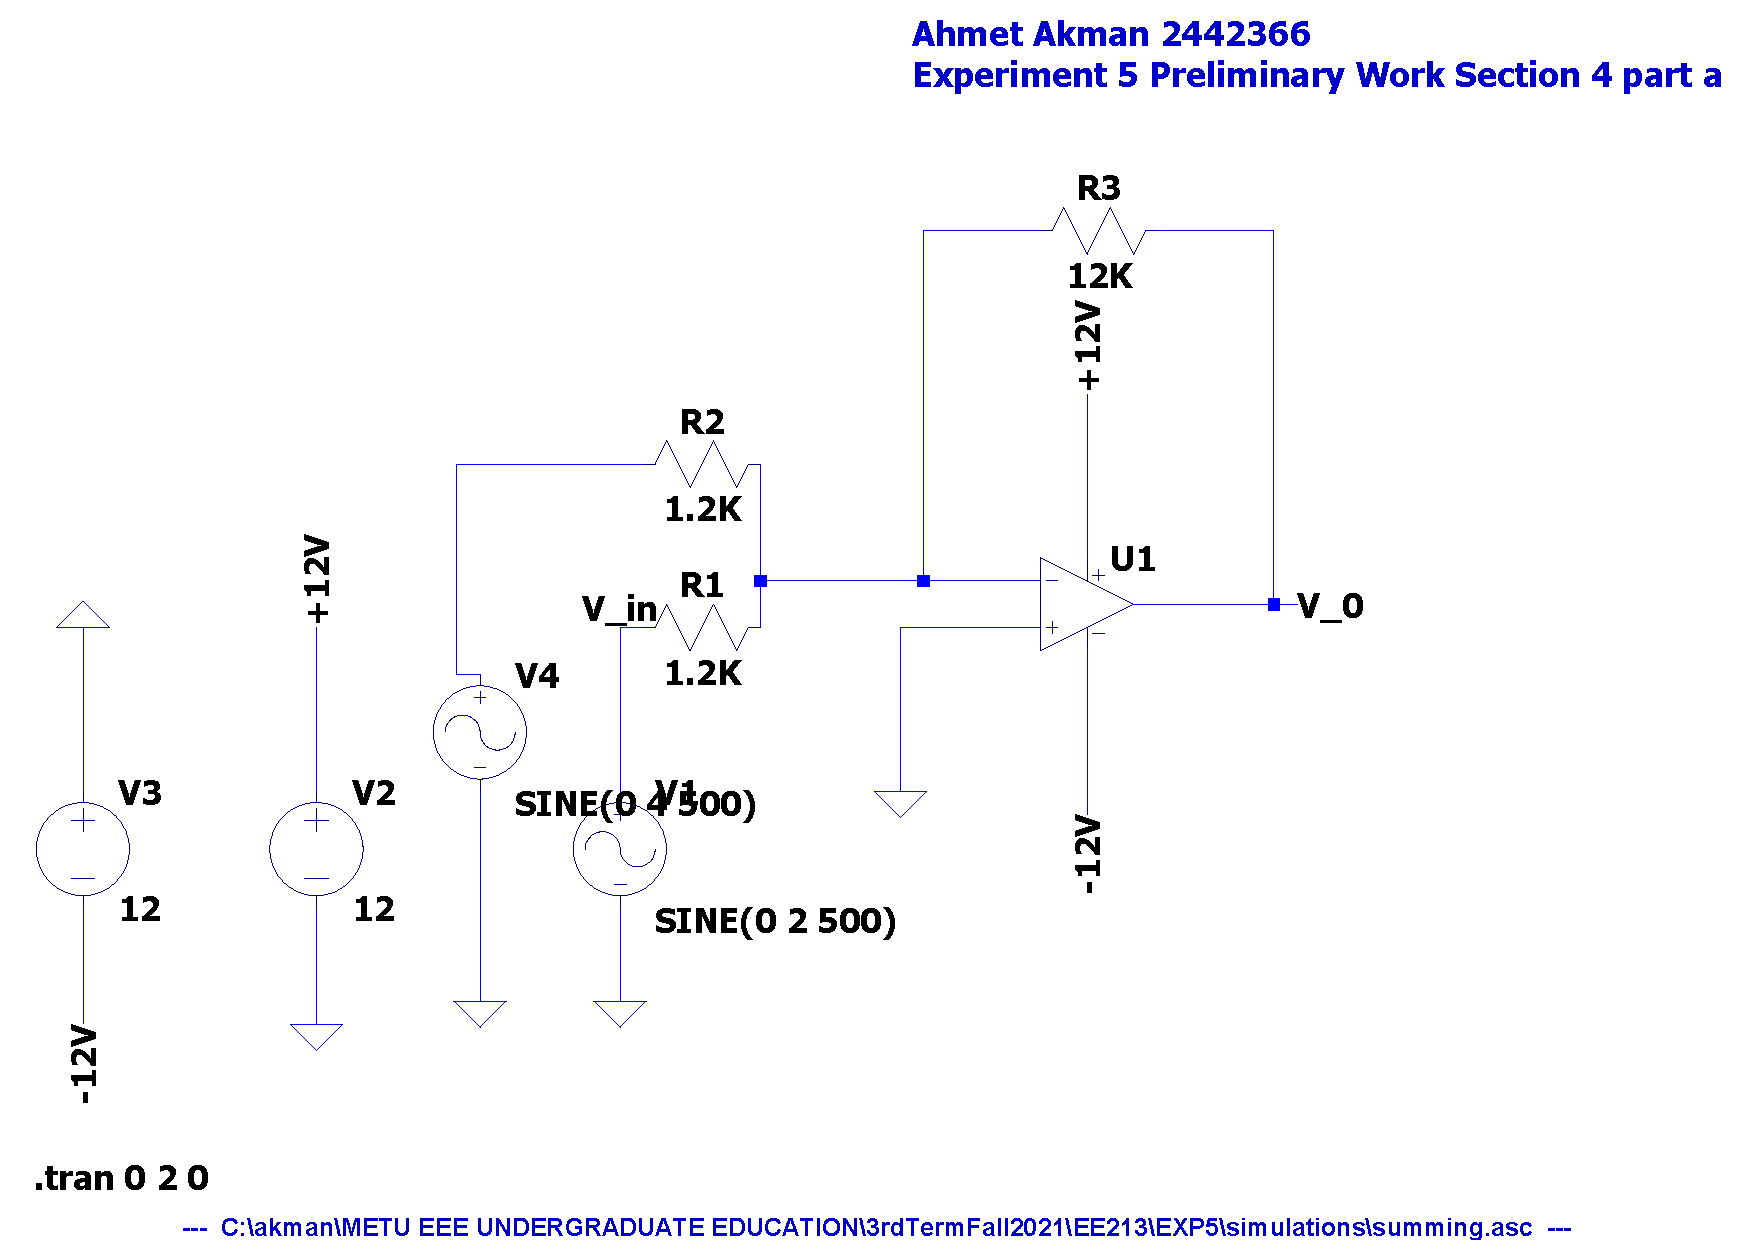
\includegraphics[width=0.8\textwidth]{summing_SCH.pdf}
   \caption{Circuit schematic for the summing amplifier.}
\end{figure} 
Then plots given in Figure 21 is obtained.
\begin{figure}[H]
	\centering
   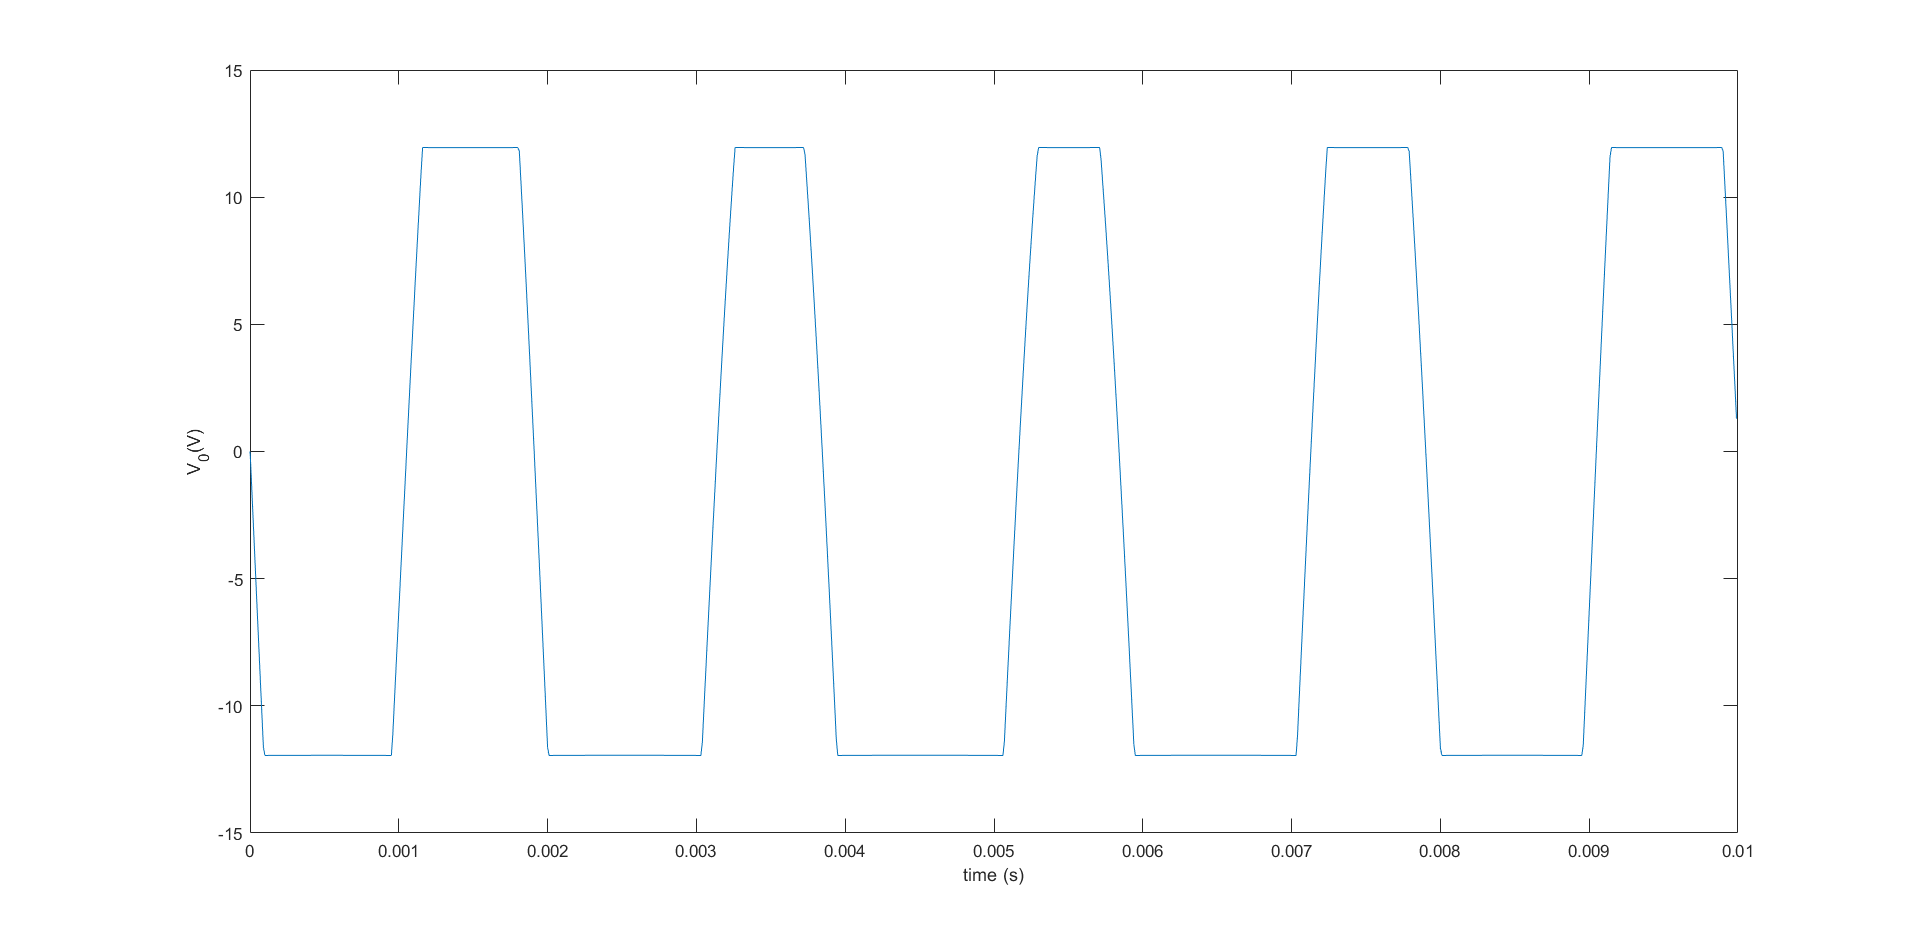
\includegraphics[width=1\textwidth]{4a_vs_t.png}
   \caption{\(V_0\) vs t}
\end{figure}


\subsection{b)}
Difference amplifier circuit is constructed in LTSpice environment. The schematic is given in the Figure 22.
\begin{figure}[H]
	\centering
   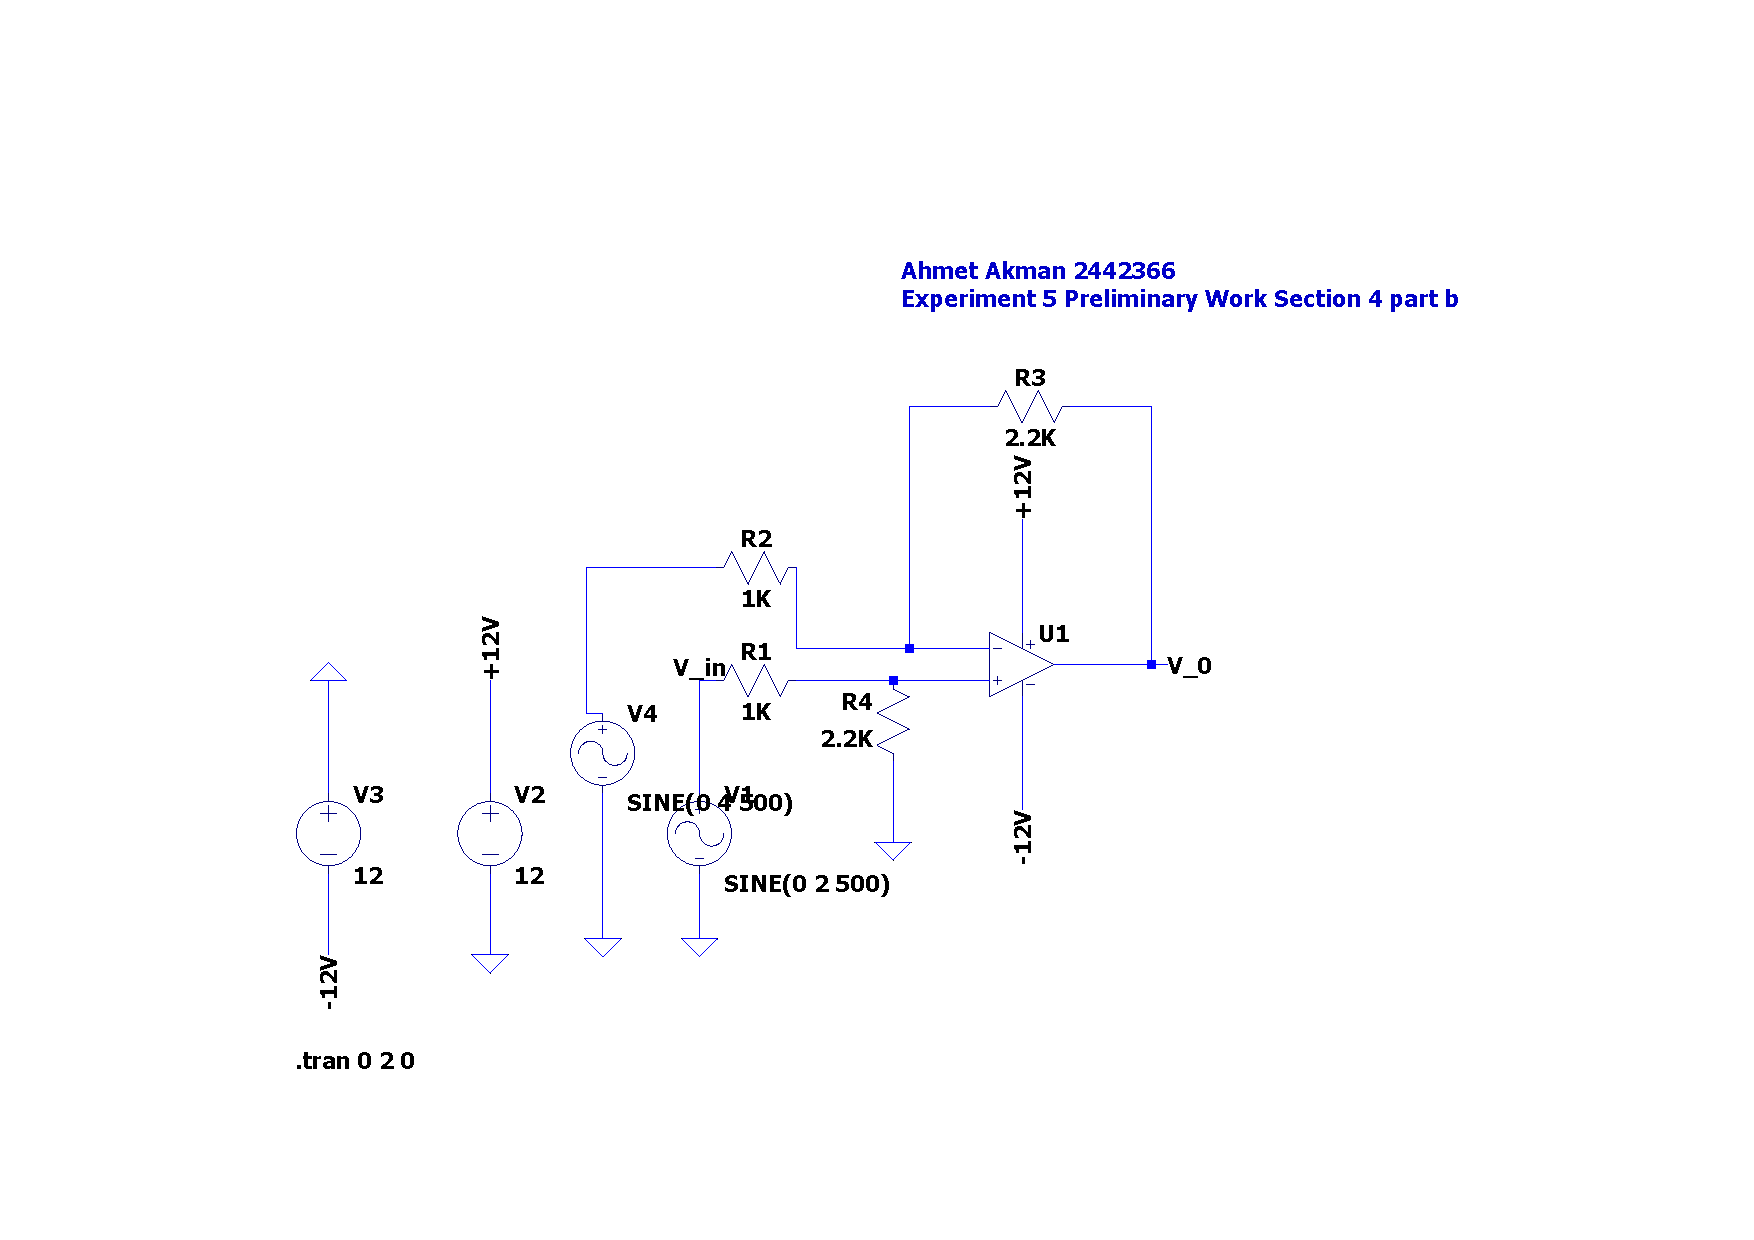
\includegraphics[width=0.8\textwidth]{difference_SCH.pdf}
   \caption{Circuit schematic for the difference amplifier.}
\end{figure} 
Then plots given in Figure 23 is obtained.
\begin{figure}[H]
	\centering
   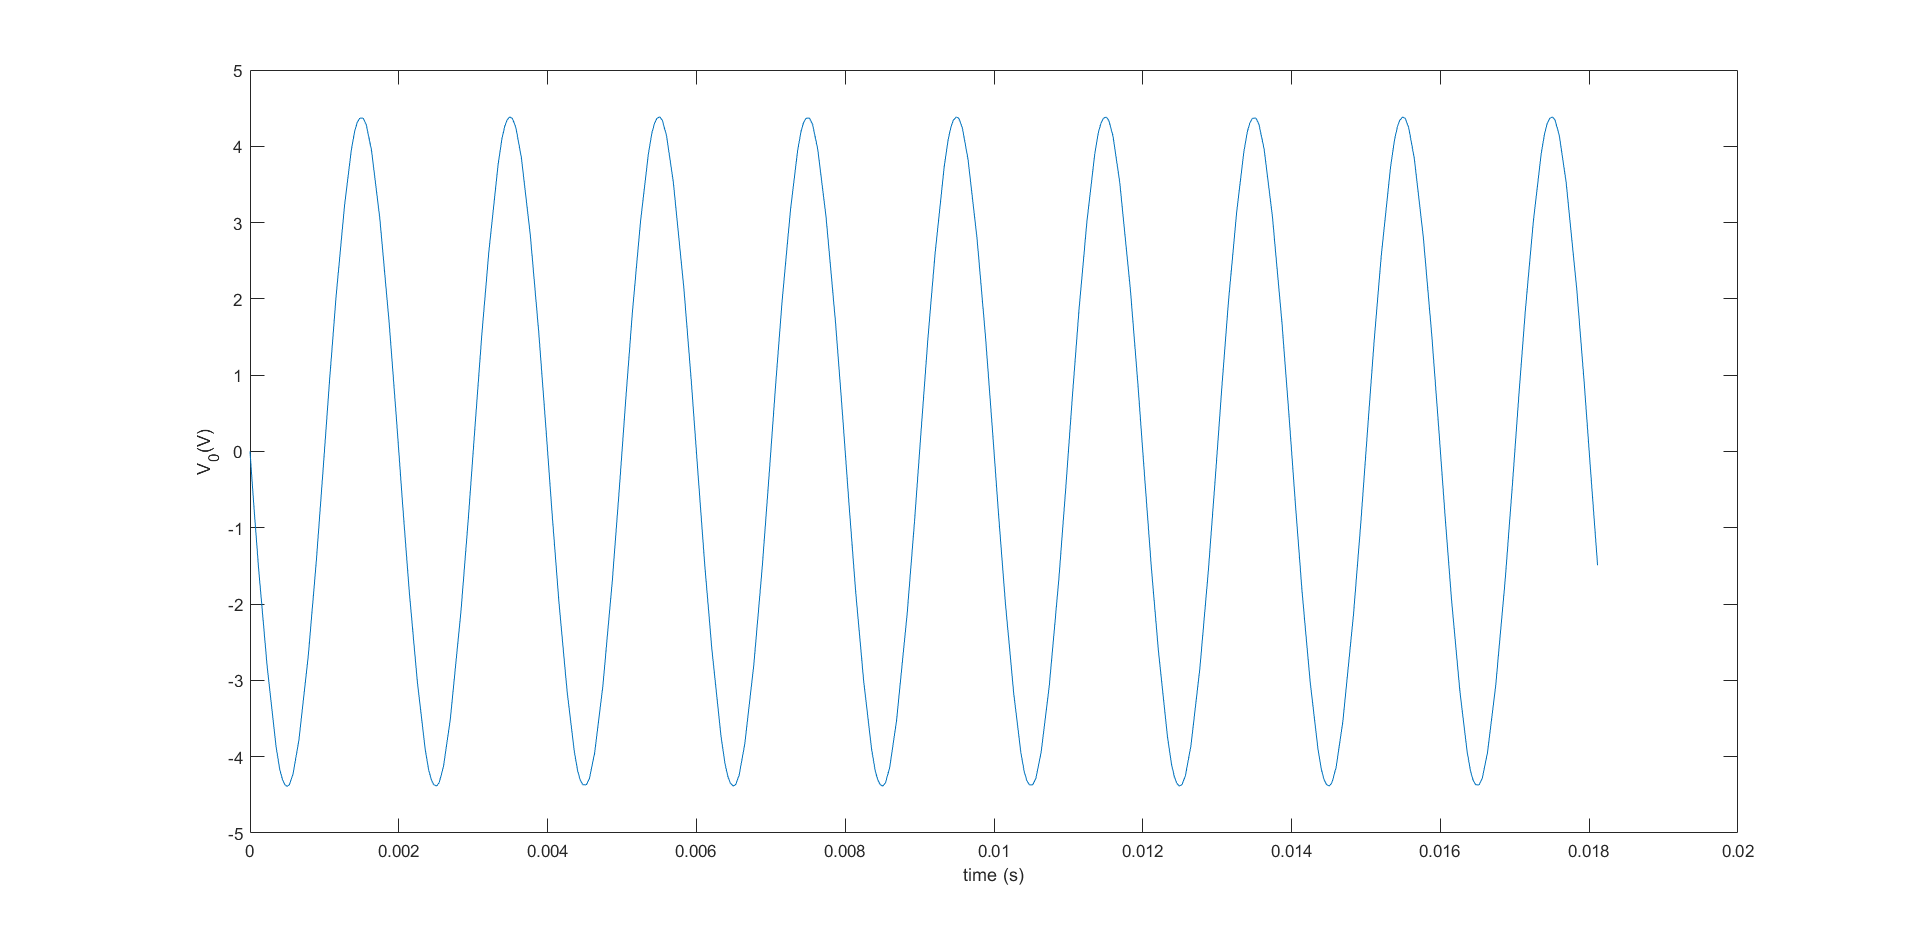
\includegraphics[width=1\textwidth]{4b_vs_t.png}
   \caption{\(V_0\) vs t}
\end{figure}
\section{Step 5}
To obtain the expression relating the output voltage \(V_0 (t)\) to the input voltage \(V_{in} (t)\) of a inverting amplifier setup, the circuit in Figure 8 is taken as the reference. Then current throught input terminals and the voltage of those terminals are taken as 0 since it is ideal amplifier. So the circuit simplifies to 2 terminals and 2 resistors. Then the following simplifications are followed.
\[\frac{V{in} - 0 }{R_1} = i\]
\[\frac{0 - V{o} }{R_2} = i\]
So, the relation becomes as,
\[\frac{V{out}}{V{in}} = -\frac{R_2}{R_1}\]
Therefore it seems the plot given in Figure 5 approximately corresponds our findings.

\section{Conclusion}
In conclusion, in preliminary work of experiment 5, "Operational Amplifiers"  needed simulation are made and necesseray data are plotted. Then the expreession for the inverting amplifier obtained and compared.
%++++++++++++++++++++++++++++++++++++++++
% References section will be created automatically 
% with inclusion of "thebibliography" environment
% as it shown below. See text starting with line
% \begin{thebibliography}{99}
% Note: with this approach it is YOUR responsibility to put them in order
% of appearance.

%\begin{thebibliography}{99}

%https://tr.overleaf.com/latex/templates/sample-lab-report-for-u-of-r-phys-349/pgsyqngcyjxk

%\end{thebibliography}


\end{document}


\begin{table}[H]
	\begin{center}
		\caption{Resistance reading by color code convention.}
		\vspace{2mm}
		\begin{tabular}{||c | c | c||} 
		 \hline
		 Color Order & Value & Tolerance \\ [0.5ex] 
		 \hline\hline
		 Brown / Black / Red / Gold & 1k\( \Omega \) & \( \% \) 5  \\ 
		 \hline
		 Yellow / Violet / Red / Gold & 4.7k\( \Omega \) & \( \% \) 5   \\
		 \hline
		 Brown / Grey / Orange / Gold & 18k\( \Omega \) & \( \% \) 5  \\ [1ex] 
		 \hline
		\end{tabular}
	\end{center}
	\end{table}

	\begin{figure}[H]
 		\centering
		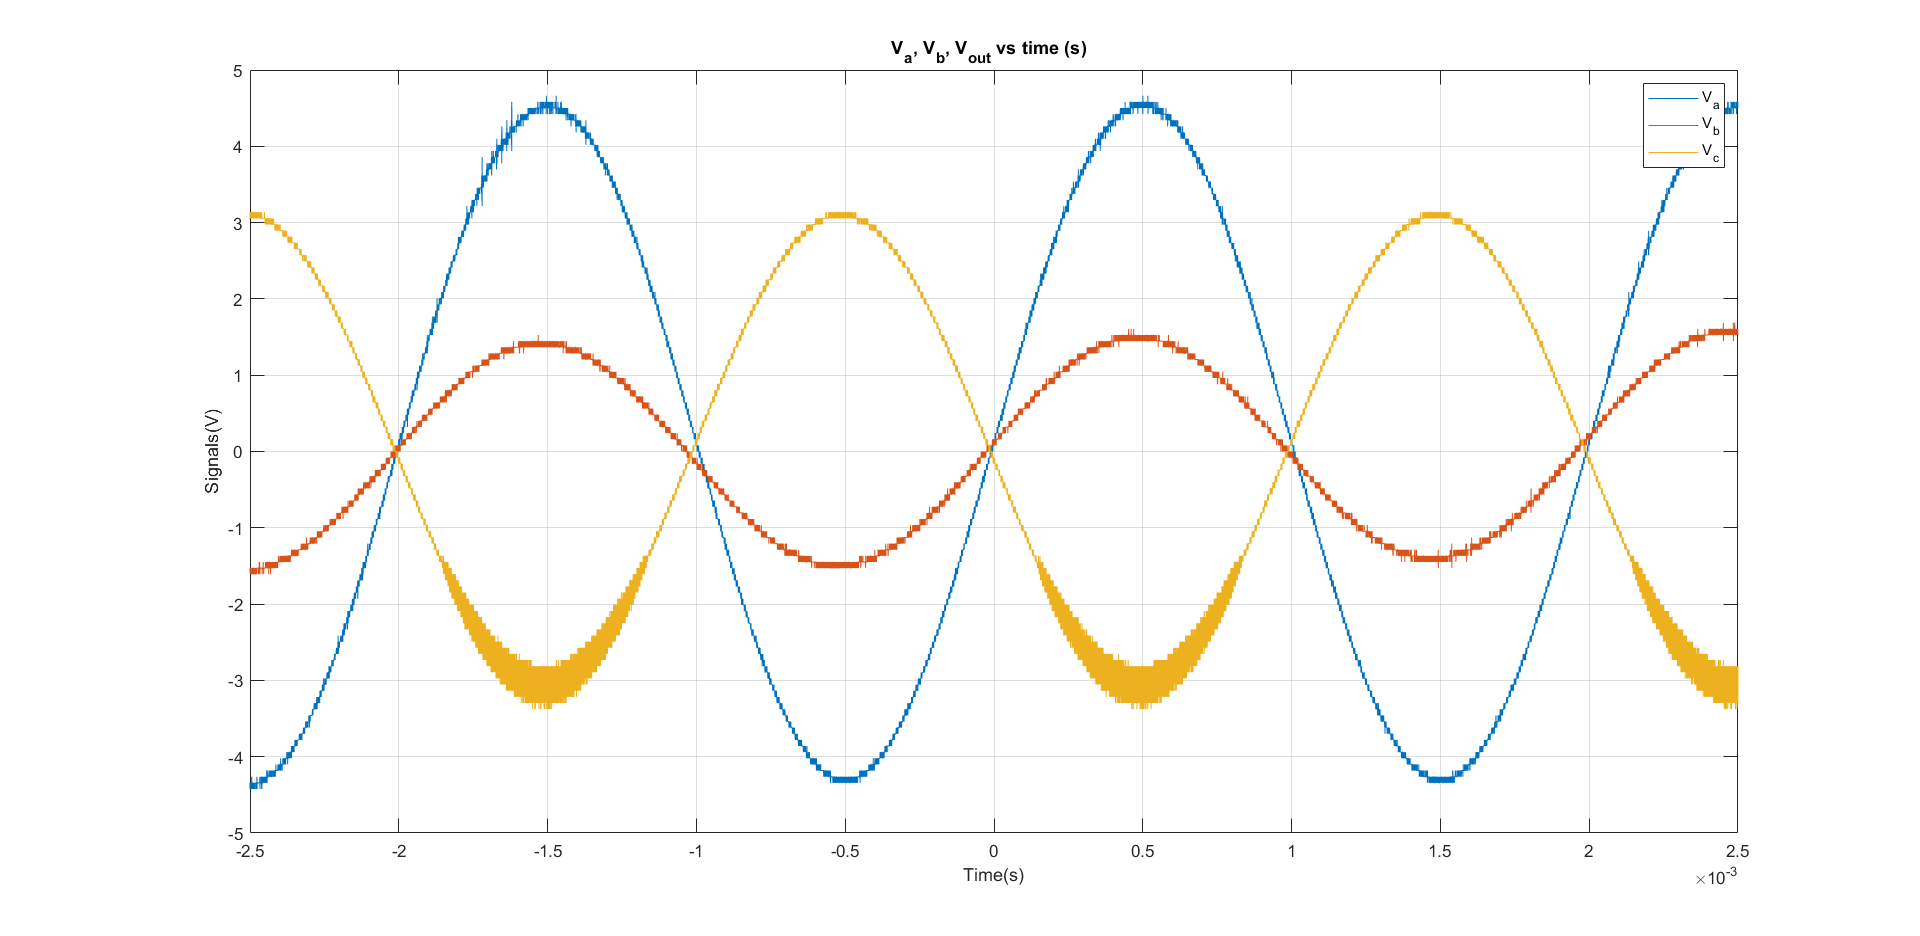
\includegraphics[width=0.6\textwidth]{5.png}
		\caption{Circuit schematic for the step 5}
	\end{figure} 

	\begin{figure}[htp] \centering{
		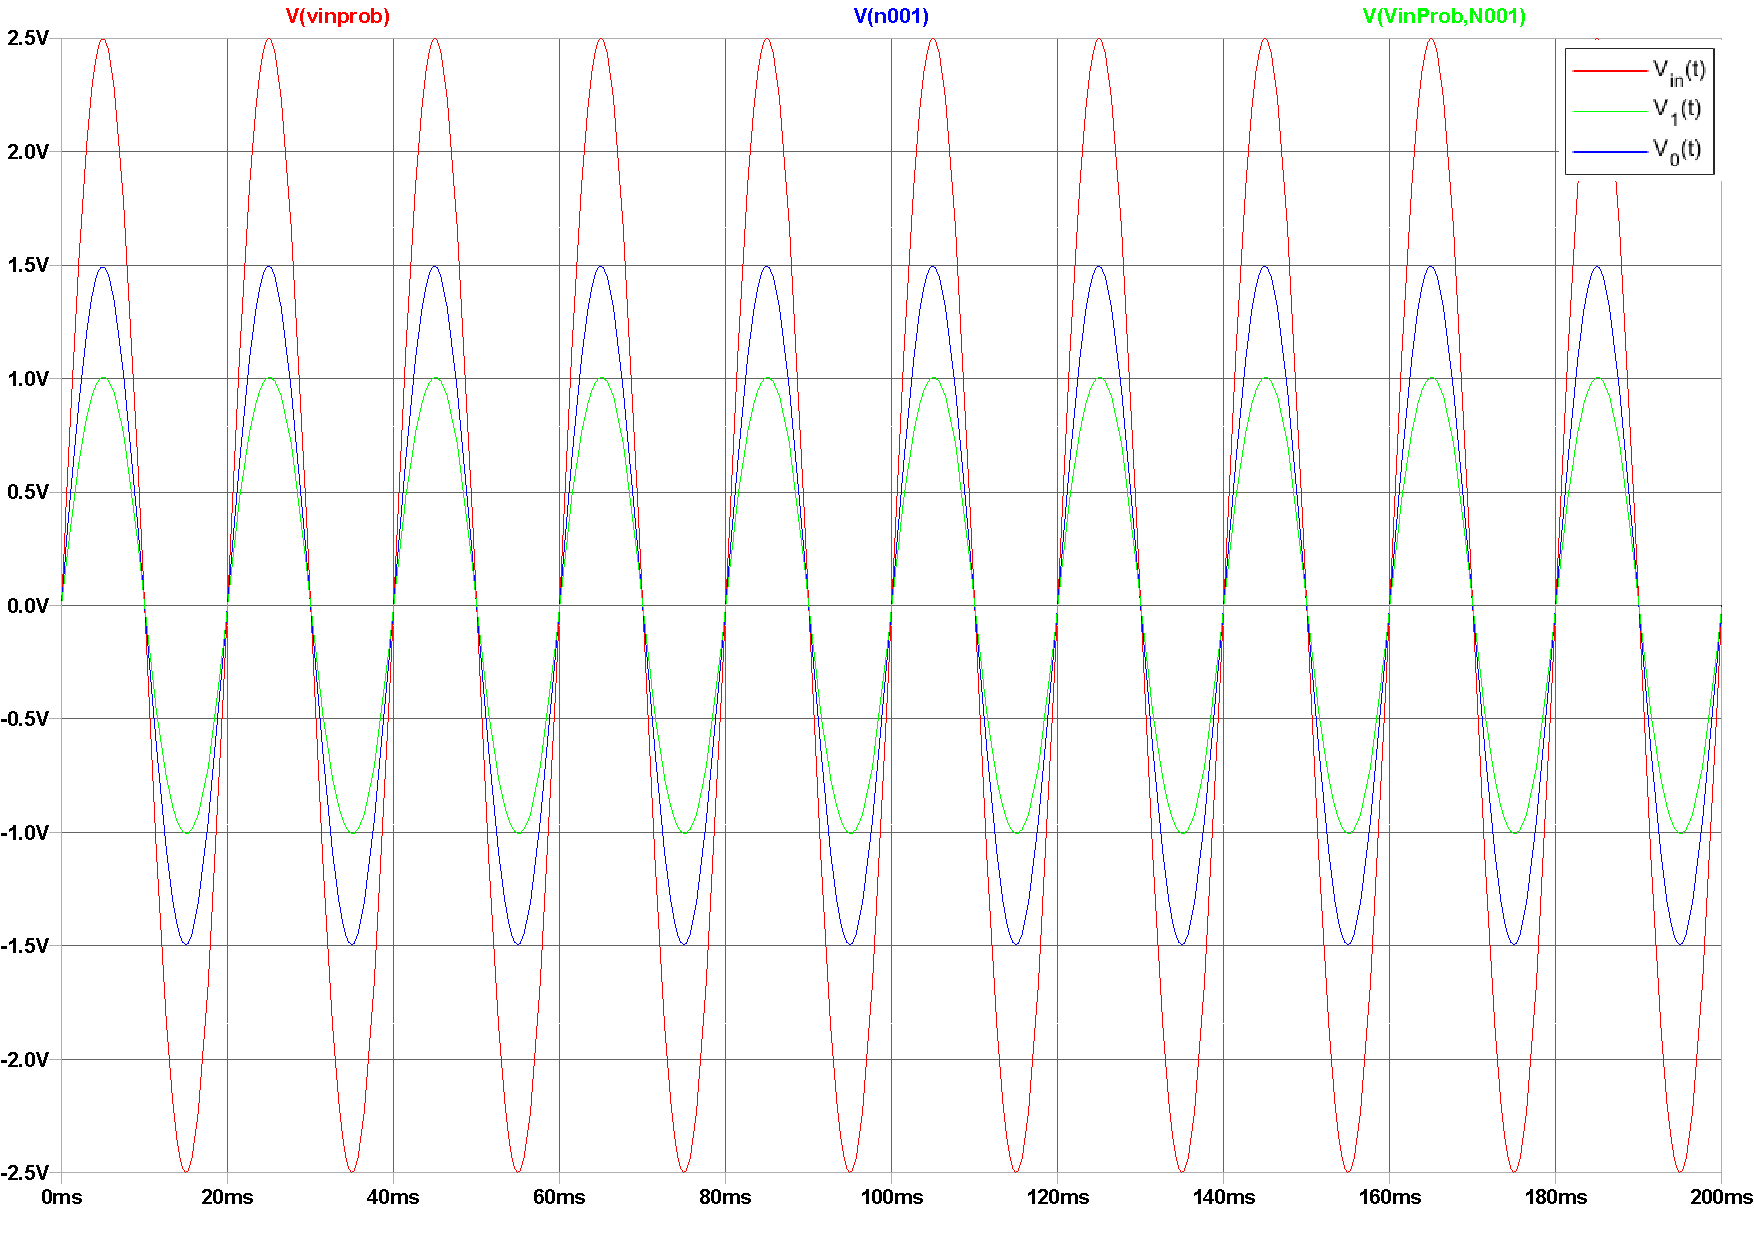
\includegraphics[scale=0.25]{2a_plot.pdf}}
		\caption{Experiment 2}
\end{figure}
	